\documentclass{article}
\usepackage[dblblindworkshop]{neurips_2026}
\workshoptitle{Agentic AI for Biological Discovery (AgenticLS)}
\usepackage[utf8]{inputenc}
\usepackage[T1]{fontenc}
\usepackage{amsmath,amssymb,booktabs,graphicx,array,microtype}
\usepackage{hyperref,url,placeins}
\newcolumntype{P}[1]{>{\raggedright\arraybackslash}p{#1}}
\title{Position: Toward a Computational Theory of Scientific Discovery}
\author{Anonymous authors}
\hypersetup{hidelinks,pdftitle={Position: Toward a Computational Theory of Scientific Discovery},pdfauthor={},pdfsubject={SUBMISSION\_CANDIDATE; AgenticLS at NeurIPS 2026; anonymous full position paper}}
\begin{document}
\maketitle
\begin{abstract}
As AI improves, which scientific problems become solvable next, and when? In a hypothetical assay comparison, the first procedure to become available can be less likely to deliver a result by a common deadline. We argue that a computational theory of scientific discovery should therefore connect capability growth to target success, procedure availability, and validated completion. Two retrospective studies test whether information about the target improves forecasts. Across 73 models and two reasoning families, object count improves pooled prediction but worsens prediction of larger deduction tasks; it does not isolate computational complexity. In 550 chemical-table replays, early outcome summaries worsen forecasts for the original easy hit criterion. They help with a stricter criterion at the shorter observation budget, but that advantage reverses at the longer budget. Fitting each budget separately does not remove that reversal. Agreement with the overall success rate also conceals opposing errors across chemical sources. Conditional calculations explain which measurements constrain availability dates and why validation and evaluation costs matter. Together, these comparisons motivate a research programme for choosing informative measurements and comparing research procedures; prospective completion dates remain unvalidated.
\end{abstract}
\section{Introduction}
As AI progresses from olympiad problems to research proofs, what changes in our expectations about an open conjecture, an unsolved algorithmic problem, or a cancer treatment? Predicting what comes next requires knowing which target requirements a system can meet and what validation remains. This question arises within mathematics as well as between mathematics and biomedicine.

Consider a procedure that selects a compound and tests it in a specified cell assay. A mathematical breakthrough alone does not tell us how reliably this procedure will find a confirmed hit. Even if that reliability can be predicted, two further questions remain: when will a suitable procedure become available, and when will selection and validation finish? The procedure available first need not be most likely to finish by a deadline (\S\ref{sec:domains}). This comparison is hypothetical; patient benefit requires a different target.

Our position is that a computational theory of scientific discovery should connect capability growth to the changing set of achievable targets and to their eventual completion. We first need a target response: how measured capability relates to the chance of validated success. Combining that response with a scenario for future capabilities and resources gives an availability date. Deployment and validation then determine completion. A breakthrough can inform the target response without settling these later stages. Researchers need target measurements before extrapolation and validation schedules before choosing a procedure. An unknown date does not mean the target is unsolvable.

The assay example supplies exact calculations of measurement and evaluation costs (\S\S\ref{sec:horizons}--\ref{sec:tests}). Two archive studies ask whether task structure or early experimental outcomes improve prediction (\S\S\ref{sec:pathways},\ref{sec:scope}). Their gains and reversals show why added information must be tested on the intended targets. These conditional examples and retrospective tests do not validate a calendar of breakthroughs.

These foundations are established: complexity and learning theory separate computation from information requirements \citep{arorabarak2007,shalev2014,traub1988}; observational scaling predicts downstream performance from capability coordinates \citep{ruan2024}; Sloth connects latent skills to model size and training tokens \citep{polo2025sloth}. ADeLe uses annotated task demands \citep{zhou2026scales}; other predictors use performance histories and validation loss \citep{hu2026neuneu,truong2026irsl}. Capability theories, measurement validity and biomedical acceleration constraints also precede this work \citep{jo2026,wallach2025,hebenstreit2026}. Our synthesis connects these established tools to the choice of scientific procedure and tests where extra target information helps. It introduces no new scaling law: a response model combined with the correct deployment model already implements this position.

\section{Defining the target and its conditions}
\label{sec:complexity}
\subsection{Define the scientific event and its resources}
A target $Q$ specifies the problem or instance population and the validated outcome to be produced. Its success probability can refer to two settings. For a declared distribution of problem instances, success is averaged over those instances. For one fixed problem, the probability instead concerns randomness in the procedure and its observations.

For the assay, fix a cell line, viability threshold and repeat-assay confirmation rule before selecting compounds. The target is one compound meeting that rule; an attempt includes selection and validation. A correct candidate somewhere in a generated set does not establish that the procedure can select and validate it \citep{dorner2026roc}. A causal mechanism or patient benefit would be a different target. Likewise, proving a supplied statement differs from selecting and resolving a significant open conjecture. 

To retain trade-offs between computation, observations and time, we record resource combinations. Let $K$ denote information and observation access, $\Pi$ the permitted procedures, and $\mathbf b$ the resource allowance. A procedure includes its model, tools, orchestration and human assistance. Comparing complete systems permits these to vary; attributing a gain to one component requires controlling the others. For procedure $\pi$, write $p(\pi,Q;\mathbf b,K)$ for its probability of producing a validated result within those limits. At required reliability $q$, define
\begin{equation}
 \mathcal B_Q(q\mid K,\Pi)=\{\mathbf b:\exists\pi\in\Pi,\ p(\pi,Q;\mathbf b,K)\ge q\},\qquad
 \mathcal A_t(q)=\{Q:\mathbf b(t)\in\mathcal B_Q(q\mid K_t,\Pi_t)\}.
 \label{eq:complexityset}
\end{equation}
\label{eq:attainable}
The first set contains sufficient resource combinations; the second gives achievable targets under resources $\mathbf b(t)$, information $K_t$ and procedures $\Pi_t$ available at time $t$. In the assay example, computation, allowed assays and elapsed validation time are separate resources. More computation may help select candidates without reducing the duration of their assays. The allowance includes campaign duration, so achievable at time $t$ means a suitable campaign can begin then, not that it has already finished. 

If two procedures need (10 compute units, 10 observations) and (100, 1), their separate minima do not imply that (10, 1) suffices. Existence of a suitable procedure does not mean an evaluator finds it. Inherent computational complexity instead concerns all algorithms in a specified model, often asymptotically. Today's model failure establishes neither an inherent lower bound nor a date for overcoming it.

Required reliability $q$ is a decision requirement, not a complexity estimate. Its choice must reflect the consequences of failure. Mean quality cannot replace success probability, which depends on the validation and selection procedures and their errors.

\subsection{Observation access changes the attainable set}
Some targets require information that the allowed observations cannot supply. Suppose two mechanisms generate identical distributions of observation histories under every permitted adaptive policy, but require opposite binary answers. Every permitted procedure then has the same output distribution in both worlds: choosing one answer with probability $r$ gives accuracies $r$ and $1-r$. Worst-case accuracy is at most $1/2$. This premise constrains every procedure; poor performance by one predictor does not establish it. Distinguishing observations or a justified structural restriction can remove this obstruction; more computation on unchanged evidence cannot. This is an identification argument under explicit observation restrictions, with close connections to causal transport and biological context \citep{bareinboim2016,dibaeinia2026,mccormick2026}.

For example, recover the program $f_a(x)=ax\bmod 2^n$ with uniformly hidden odd $a$. If each rejected candidate only rules out its own coefficient, positive verification with 90\% probability needs $\lceil.9\,2^{n-1}\rceil$ checks. Observing $f_a(1)$ instead reveals $a$. The exponential cost belongs to the restricted interface, not multiplication. Appendix~\ref{app:synthesis} supplies exhaustive checks and verification costs.

\section{From demonstrated capability to target performance}
\label{sec:pathways}
A source score describes a system; it does not describe what a new target demands. We ask whether combining the two improves prediction. A solved problem can reveal relevant ability without transferring its solution. Let $\mathbf z$ be the measured capability profile and $\boldsymbol\kappa_Q(K)$ the target description under access $K$. A shared rule $F_{\boldsymbol\theta}$, with fitted parameters $\boldsymbol\theta$, predicts success from these quantities and the resource allowance. For the assay target, success means one complete selection-and-validation attempt. Our archive tests instead use computational outcomes. The second expression is a restricted logistic example:
\begin{equation}
 \widehat p_Q=F_{\boldsymbol\theta}(\mathbf z,\boldsymbol\kappa_Q(K),\mathbf b),\qquad
 \widehat p_Q=\sigma(\mathbf a_Q^\top\mathbf z-d_Q),\quad \sigma(u)=(1+e^{-u})^{-1}.
 \label{eq:bridge}
\end{equation}
\label{eq:logistic}
The logistic model holds resources, information and protocol fixed. Log-odds are $\log[p/(1-p)]$; a linear relation on this scale becomes a curved probability response. The weights $\mathbf a_Q$ describe how target log-odds vary with measured capabilities; $d_Q$ shifts the response curve. This item-difficulty parameter is not computational complexity. Fix capability units and normalization before comparing coefficients.

For an unseen target, shared functions must determine its coefficients: $\mathbf a_Q=\mathbf a_{\boldsymbol\theta}(\boldsymbol\kappa_Q)$ and $d_Q=d_{\boldsymbol\theta}(\boldsymbol\kappa_Q)$. Fitting separate coefficients after observing each target's outcomes cannot supply that prediction. Even a successful shared fit remains an association: it does not establish that intervening on one capability causes improvement.

\subsection{Testing target descriptions in a common archive}
We use the public ObsScaling archive \citep{ruan2024}. Principal component analysis (PCA) summarizes seven source scores: MMLU, ARC-C, HellaSwag, Winograd, TruthfulQA, GSM8K and XWinograd. PC1 is the first coordinate; PC1--3 uses the first three. Source scores and PC coordinates are standardized on training models only. 

We test a narrower version of the shared-description hypothesis using BIG-Bench Hard (BBH) logical deduction and shuffled-object tracking, each with 3, 5 and 7 objects. The descriptor is log object count, fixed from task definitions. Three-shot chain-of-thought strict-match scores come from the same archive: 73 models in 20 archive-defined groups, each evaluated on six task versions, giving 438 aggregate success rates. These 20 archive groups can share ancestry; their identities are listed in Appendix~\ref{app:empirical}. A cell is a published model--task rate, not one generated answer. We compare PC1 and PC1--3 with count-informed predictors. Adding count shifts predicted log-odds; interactions additionally let capability effects vary with count.

PCA uses each training model once; regressions fit its rates on the available task versions. Prediction inputs are seven measured source scores and, for count-informed fits, target object count. Family labels define exclusions; only the task-family-mean baseline uses task identity as a prediction key. Test rates are withheld. We score predictions by mean squared error against archived success fractions (rate-MSE), not by counting validated discoveries. Table~\ref{tab:descriptor} separates task-family, model-family and size holdouts from joint family exclusion.

\begin{table}[htbp]
\centering\small
\caption{Archived rate-MSE; lower is better. Separate holdouts exclude a task family (438 cells), model family (438), or size 7 (146; training at 3/5). Joint holdout excludes both families (438 cells); Cells weights cells equally, Families weights the 20 model groups equally. Each split uses identical cells across predictors. $\dagger$ marks post-result rivals; the joint test is also post-result. These are retrospective, not contamination-controlled tests.}
\label{tab:descriptor}
\begin{tabular}{lrrrrr}
\toprule
& \multicolumn{3}{c}{Separate holdouts} & \multicolumn{2}{c}{Joint holdout}\\
Predictor & Task & Model & Size & Cells & Families\\
\midrule
Pooled mean & 0.0431 & 0.0427 & 0.0446 & 0.0446 & 0.0532\\
Task-family mean & 0.0431 & 0.0422 & 0.0447 & 0.0446 & 0.0532\\
PC1 & 0.0342 & 0.0320 & 0.0307 & 0.0357 & 0.0432\\
PC1--3 & 0.0355 & 0.0330 & 0.0307 & 0.0379 & 0.0459\\
Count only$^\dagger$ & 0.0395 & 0.0371 & 0.0279 & 0.0410 & 0.0535\\
PC1--3 + count$^\dagger$ & 0.0260 & 0.0234 & 0.0179 & 0.0285 & 0.0356\\
PC1--3 + chance floor$^\dagger$ & 0.0266 & 0.0270 & 0.0217 & 0.0287 & 0.0350\\
PC1--3 + count interactions & 0.0277 & 0.0238 & 0.0195 & 0.0301 & 0.0377\\
\bottomrule
\end{tabular}

\end{table}

In Table~\ref{tab:descriptor}, PC1--3 + count outperforms the interaction model in the three separate holdouts. The chance-floor predictor uses $1/n+(1-1/n)\sigma(\beta_0+\boldsymbol\beta^\top\mathbf z)$ for $n$ objects; it assumes rather than guarantees a floor on LLM accuracy. The task-family mean uses training rates from the same task family, falling back to the pooled mean when that family is withheld. Among these eight, the chance-floor predictor has the lowest task-family cross-entropy (Appendix~\ref{app:empirical}); no new models were evaluated.

\paragraph{One held-out prediction.}
To predict Gemma-7B's seven-object deduction score, we withhold its model group, the deduction family and size 7, then train on 142 tracking rates: 71 non-Gemma models from 19 groups, at 3/5 objects. Gemma-7B's source scores and the target count enter the fitted rule; its deduction outcome does not. PC1--3 predicts $.411$; adding count predicts $.211$. The archived rate is $.376$, giving squared errors $.00120$ and $.02720$. This example shows how one prediction is scored; it does not represent the average effect. Figure~\ref{fig:joint_main} summarizes all such exclusions, including the pooled benefit and deduction reversal.

\begin{figure}[htbp]\centering
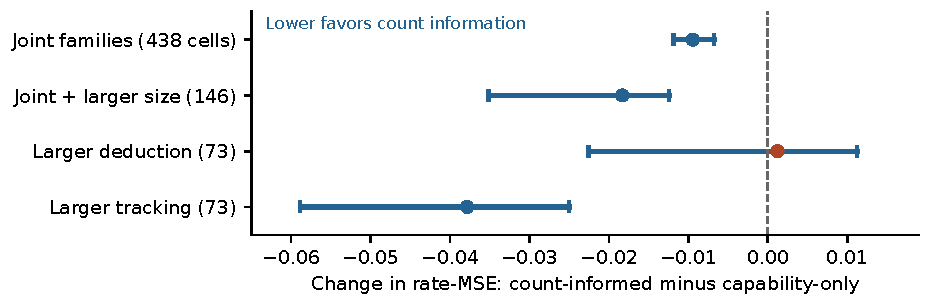
\includegraphics[width=\linewidth]{figures/joint_effects_main.pdf}
\caption{Does object count improve prediction when both model and task families are withheld? Dots show the rate-MSE of PC1--3 + count minus that of PC1--3; negative favors adding count. Bars are 95\% percentile ranges from 500 model-family refits, not uncertainty over new task families. The last two rows partition the 146-cell size-extrapolation test. Deduction worsens at the observed point estimate and its interval spans zero.}
\label{fig:joint_main}
\end{figure}

PC/count fits minimize the sum of squared residuals on logits of target rates clipped to $[.005,.995]$, plus the sum of squared non-intercept coefficients (ridge penalty 1). Log count is standardized on training cells. Coefficients are shared across task versions; the intercept is unpenalized. The penalty is fixed, not tuned on held-out outcomes.

At seven objects, adding count changes tracking rate-MSE from $.06159$ to $.02375$, but deduction from $.01680$ to $.01802$ (73 cells each; Figure~\ref{fig:joint_main}). This establishes a target-description association, not a computational-complexity mechanism: count also changes the answer space. A forecast for a new target needs a relevant transfer test, not just a better pooled score.

The preferred predictor also depends on whom the average represents. In Table~\ref{tab:descriptor}, additive count narrowly beats the chance floor when cells receive equal weight ($.02845$ vs. $.02873$), but loses when each model family gets weight $1/20$ ($.03558$ vs. $.03503$). Rankings therefore depend on the error measure, weighting and holdout. The pooled count gain survives alternative fits (probit, direct rate prediction, clipping thresholds and a quadratic capability-only rival), but adding count to the chance-floor predictor is not uniformly better.

Figure~\ref{fig:joint_main}'s ranges concern model-family sensitivity with two fixed task families and no item-level outcomes (Appendix~\ref{app:robustness}). A date forecast additionally needs a capability-growth trajectory.

\section{From target performance to a conditional date}
\label{sec:horizons}
\subsection{The missing relation and how to measure it}
A response curve gives success at a capability level; a date asks when that procedure becomes available. For the assay, require a complete single-candidate procedure to pass with probability at least $q$, rather than reaching $q$ through many attempts. For fixed reliability and a development scenario, define the earliest availability time as
\begin{equation}
 \tau_Q(q)=\inf\{t\ge0:Q\in\mathcal A_t(q)\}.
 \label{eq:horizon}
\end{equation}
If no permitted procedure ever meets the target, $\tau_Q=\infty$. This date concerns availability; a campaign need not start then. Each scenario below permits one procedure; admitting alternatives cannot delay the earliest availability date. A probabilistic forecast would also need uncertainty about capability growth, target response, resources and access.

The following values are hypothetical. Here $p_Q$ is single-attempt success and $q$ its required threshold; $\lambda$ measures log-odds change per capability unit, $v$ capability units per year, and $\tau_Q$ years to availability. Section~\ref{sec:tests} instead uses $\rho$ for a multi-attempt campaign hit probability. With initial log-odds $\eta_0$ and a fixed linear relation,
\begin{equation}
 \operatorname{logit}p_Q(t)=\eta_0+\lambda vt,\qquad
 \tau_Q(q)=\frac{\operatorname{logit}q-\eta_0}{\lambda v}.
 \label{eq:crossing}
\end{equation}
The finite crossing formula assumes $v,\lambda>0$ and initial success below $q$. With $\eta_0=-3$, $v=1$ and $q=.8$, procedures A and B with slopes (couplings) $\lambda=1$ and $.5$ become available after 4.39 and 8.77 scenario-years; a zero-coupling procedure never does. All three agree on the source trajectory and current target success $.0474$. At one additional source unit, A and B instead predict $.1192$ and $.0759$: a matched target measurement can begin to distinguish them, subject to sampling error. Thus source progress and current target performance do not identify the horizon when coupling is unrestricted. Appendix Figure~\ref{fig:horizons} displays these constructed curves. 



\paragraph{A constructive measurement procedure.}
Measuring the target at two capability levels supplies information missing from a single current success rate. Assume log-odds vary linearly with capability. Use the same target protocol at levels separated by $\Delta>0$, with $N$ independent success/failure trials at each level. Form individual 97.5\% Clopper--Pearson intervals $[L_0,U_0]$ and $[L_1,U_1]$ by allocating .0125 to each of four tails, giving at least 95\% simultaneous coverage \citep{clopper1934}.

Subscripts 0 and 1 denote lower and higher capability. To bound improvement conservatively, pair the lower success bound at higher capability ($L_1$) with the upper bound at lower capability ($U_0$); reverse the endpoints for the largest change. On the log-odds scale, dividing by the capability separation gives
\begin{equation}
 \lambda\in\left[\frac{\operatorname{logit}L_1-\operatorname{logit}U_0}{\Delta},
 \frac{\operatorname{logit}U_1-\operatorname{logit}L_0}{\Delta}\right].
 \label{eq:lambda_interval}
\end{equation}
Across repeated samples at these fixed levels, at least 95\% of intervals cover the slope if the binomial and affine-logit premises hold; this is not 95\% coverage of a future discovery date. Zero successes or all successes at a level can leave an interval endpoint infinite. Cross-level independence is unnecessary for coverage, but used for exact power calculations. The slope describes association unless capability is isolated by intervention. At observation cost $a$, measurement costs $2Na$.

We enumerate success-count pairs at sample sizes 25/100/500, initial yields .01/.05/.2, separations .5/1/2 and couplings 0/.5/1. These 81 prespecified settings check coverage and recovery, including zero coupling and low yield. With initial target success .05, true coupling 1 and separation 2, the probability of a positive lower coupling bound is 4.9\% at $N=25$, 90.7\% at $N=100$, and above 99.9\% at $N=500$ per level. At $N=100$, the median interval width is 1.69 and 0.59\% of intervals remain unbounded. The finite grid's minimum coverage is 99.81\%; the analytical union-bound argument supplies the general guarantee (Appendix~\ref{app:identification}).


At the same $N=100$, slope 1 and separation 2, reducing initial success to .01 lowers positive-slope detection to 6.585\% and leaves 36.651\% of intervals unbounded. The measurement can therefore be valid yet uninformative. In the assay example, very few validated hits at either capability level would leave the improvement rate poorly constrained even when both groups were measured correctly.

Bounding the availability date requires a positive lower slope bound, a supported growth path and continued access. Fix the endpoint, protocol and source scale before sampling; propagate joint uncertainty to the target threshold. A rising but saturating response can match both probabilities exactly and never reach the threshold (Appendix~\ref{app:twolevelboundary}). Fit on two levels, then predict a withheld third before observing it; repeat across held-out targets. This tests extrapolation beyond the fitted pair. Logistic is a starting link, not a privileged law; archive link sensitivities are retained.

Repeated trials estimate success on the declared target; they do not sample new problems. Model-family comparisons may change data, architecture and tools together. Binomial intervals do not remove these confounders: record the complete procedure and check its stability across levels.

\subsection{Why accurate performance fits can give poor dates}
Near a plateau, a small error in predicted success can imply a large error in the date it reaches a threshold. The response slope determines that conversion. If true target log-odds $\ell(t)$ have derivative at least $m>0$ throughout an interval containing both the true and predicted crossings, and predicted log-odds have uniform error at most $\varepsilon$ there, then
\begin{equation}
 |\widehat\tau-\tau|\le\varepsilon/m.
 \label{eq:timeerror}
\end{equation}
At the predicted crossing, the true log-odds are at most $\varepsilon$ from the threshold. A slope of at least $m$ forces that gap to close within $\varepsilon/m$ time units (Appendix~\ref{app:horizonproofs}). A log-odds error of $.2$ thus allows $.2$ years at slope 1 per year, but 2 years at slope $.1$. The difficulty is establishing uniform error and positive growth over the relevant future interval. Pointwise fitted-curve intervals do not establish either premise.

\section{From availability to validated completion}
\label{sec:domains}
Return to the assay target. A confirmed hit arrives only after a campaign is launched and validation finishes; procedure availability alone does not specify completion. Let $C_Q$ be that completion time. For a fixed schedule with validation-completion dates $t_j$, let $h_j$ be the probability that campaign $j$ succeeds conditional on all preceding campaigns failing. The probability of no success is the product of these conditional failure probabilities, so
\begin{equation}
 \Pr(C_Q\le T)=1-\prod_{j:t_j\le T}(1-h_j).
 \label{eq:completionhazard}
\end{equation}
This probability identity is not a fitted scaling law: prediction still requires the conditional success probabilities under the deployment policy. Marginal scores cannot generally replace them: earlier failures may reveal a shared weakness that makes later campaigns less likely to succeed. An attempt may contain an adaptive agent workflow; independent restarts are a separate assumption. With independent serial attempts of success $p$, launch time $s$ and validation duration $d$, the expected number of attempts is $1/p$, giving mean completion $s+d/p$. \paragraph{One decision carried from capability to completion.}
Continue the hypothetical assay comparison in Section~\ref{sec:horizons}. A reaches reliability $.8$ at year 4.39; B at 8.77. Choose one procedure, launch immediately on availability, and freeze that version at success $.8$. Suppose independent serial attempts require four years of validation for A and one quarter-year for B. One validation pipeline is available; further model improvements during a campaign are excluded. By a common deadline at year 10, A completes one attempt and B completes four, giving success probabilities $.8$ and $1-(1-.8)^4=.9984$. Their mean completion times are 9.39 and 9.09 years. Choosing the earlier available procedure therefore chooses the worse completion forecast in this scenario.

At the same fixed success $q$, B has lower mean completion time precisely when $d_A-d_B>q(\tau_B-\tau_A)$. Here the duration advantage is 3.75 years, exceeding the 3.51-year boundary. Measuring validation duration can change the choice even after capability responses are known. If durations are equal, A wins; if access or attempt dependence changes, recompute the comparison. Combining the success forecast with validation duration already gives this answer; the example shows why both are needed. All values are stipulated, not biomedical forecasts.

For a fixed agent computation, let $W$ be total work and $L$ the duration of the longest chain of dependent steps. With $P$ processors, runtime satisfies $T_P\ge\max\{W/P,L\}$. If validation requires $r$ successive rounds of duration at least $\ell$, then $L\ge r\ell$. More agents can change the procedure; parallelizing unchanged work preserves its dependency chain \citep{meyerson2025,shun2024parallel,kim2026agents}. Agent-count comparisons must include context processing, coordination and validation costs. Serial-computation bounds depend on architecture \citep{liu2026serial}; human-duration horizons differ from workflow depth \citep{liu2026bridge}.

\section{Scientific targets and the cost of establishing progress}
\label{sec:tests}
\subsection{What the scientific example measures}
Co-Scientist's initial acute myeloid leukemia (AML) repurposing example has three cell-viability hits among five oncologist-selected drugs from thirty ranked proposals \citep{gottweis2026coscientist}. This is a selected-subset result for a human-assisted procedure. These selected assay hits support that source's demonstration, but do not estimate a capability--yield curve: capability levels were not paired with matched laboratory outcomes. Clinical benefit requires different validation (Appendix Table~\ref{tab:transferrecord}).

\subsection{A worked decision about future campaigns}
Establishing a procedure's advantage may itself be expensive. The following calculation separates low decision error from useful, affordable evaluation. This hypothetical pilot evaluates method selection: its attempts are charged separately and their own discoveries receive no value. Here $p$ is per-attempt success; $\rho$ is the required chance of at least one campaign hit, distinct from single-attempt reliability $q$ in Section~\ref{sec:horizons}. Independent attempts need a cap of $\lceil\log(1-\rho)/\log(1-p)\rceil$. At $p=.1$ and $\rho=.9$, this is $\lceil\log(.1)/\log(.9)\rceil=22$ attempts. At costs of 10 and 11 units per attempt, the baseline and candidate need reserves of 220 and 242: enough budget to fund their attempt caps. Doubling candidate yield to .2 reduces its cap to 11 and reserve to 121; a strict saving already occurs at approximately .1141. The pilot estimates both yields. Reserve differs from expected expenditure until first success \citep{erol2026costofpass}: the baseline averages $10/.1=100$ units with recognizable success and early stopping, although its 90\%-success cap is 220.

Take 100 independent success/failure observations per arm, with independent arms. Individual 97.5\% Clopper--Pearson yield intervals (tail probability .0125) give at least 95\% simultaneous coverage. Convert each yield interval to reserve bounds using the cap formula: lower yield needs more attempts, so it gives the upper reserve. The rule adopts only when savings hold throughout these bounds. It adopts if the candidate's upper reserve is below the baseline's lower reserve, declares non-saving if the candidate's lower reserve is at least the baseline's upper reserve, and otherwise defers. Deferral means insufficient evidence for either decision, not that the candidate cannot save resources. Zero lower yield gives an infinite upper reserve.

For example, ten baseline successes and forty candidate successes give reserve ranges $[120,520]$ and $[44,77]$ units. Even the candidate's upper bound, 77, is below the baseline's lower bound, 120: the rule adopts. Ten successes in each arm give overlapping ranges $[120,520]$ and $[132,572]$, so it defers. 

Enumerating every pair of success counts, weighted by its probability under the stipulated yields, gives exact decision frequencies rather than empirical estimates. At equal yields $.1$, comparing reserves at the observed success fractions falsely favours the candidate in 41.877\% of pilots. The interval rule falsely adopts in .018\% but leaves 99.900\% unresolved. At candidate yield $.2$, it adopts in only 4.572\%. Among resolved decisions, the error rate is 18.33\% at unchanged yield: unconditional error control does not imply 95\% correctness conditional on deciding. Always deferring gives zero false adoptions but also zero useful adoptions, without pilot cost. The interval rule must earn its cost through correct decisions, not low error alone.



At $N=1000$ and candidate yield $.20$, adoption rises to 98.503\% (Appendix Table~\ref{tab:pilotfull}), but the evaluation costs 21,000 pilot units for a true reserve saving of 99 per future campaign. Even granting perfect adoption, offsetting that cost takes 213 campaigns; this is reserve accounting, not cash payback. Appendix~\ref{app:threshold_sensitivity} reports threshold sensitivities. The illustrative rule is not optimized and establishes no intrinsic evidence-cost limit.

\section{Early experimental outcomes and forecast limits}
\label{sec:scope}
\subsection{Do early experimental outcomes improve a completion forecast?}
We replayed 550 campaigns: 50 seeds on each of eleven 512-candidate tables from four source groups: four additive-screening plates, five Buchwald--Hartwig tables, one C2-yield table and one Suzuki--Miyaura table \citep{rankovic2026}. Each campaign starts with five random observations, then selects the candidate maximizing kernel-predicted yield plus one posterior standard deviation. All candidate input features are known. The kernel is $\exp(-2d)$, where $d$ averages numeric squared distances normalized by catalogue ranges and categorical mismatches; diagonal regularization is .01. Each selection reveals one recorded outcome. Seeds vary histories on fixed tables, not independent scientific validations.

After five or ten observations (the pilot), we predict whether that campaign will find a hit by observation 20 or 40 (the total budget). All forecasts receive these counts and whether a hit has already occurred. The hit threshold is the complete table's 90th percentile: it uses unrevealed outcomes and is supplied retrospectively, not estimated from the pilot. Apart from this threshold, unrevealed yields are not predictor inputs. After a pilot hit all methods assign probability one.

Otherwise, the budget-only logistic regression uses log pilot length and log total budget; the richer predictor adds threshold-relative best and mean yields, yield dispersion and mean pairwise kernel similarity. We withhold one entire source group at a time. Fits use only no-hit pilots from the other three groups, train-only feature standardization, non-intercept ridge penalty 1, and weights balancing tables and groups. Thus the comparison tests whether early outcome summaries improve forecasts beyond campaign size, not whether more capable AI discovers better chemistry (Appendix~\ref{app:finite_table}).

Brier score measures squared probability error against the campaign's binary outcome, averaging tables within source groups and then groups equally. After five observations, forecasting a hit by observation 20 gives .01862 with summaries versus .01773 for budget-only (lower is better). Among 329 campaigns without a pilot hit, scores are .03253 versus .03106. Neither comparison favors the richer predictor. The group-averaged hit rate reaches 98.2\% by budget 20; every retained campaign hits by 40. Later checks give Brier scores .01774 for the success rate estimated from training groups (prevalence) and .01800 for always predicting success. Always-success is worse on log-loss. This endpoint limits discrimination; the replay establishes no wet-lab discovery.

\paragraph{Does a stricter endpoint change the conclusion?}
After observing near-universal success, we compared the original 90th-percentile endpoint with stricter 95th and 99th percentiles, keeping the same trajectories and source exclusions. Changing the endpoint changes hit labels, pilot-hit status and threshold-relative features, while the search policy stays fixed. At the 99th percentile and budget 20, summaries outperform budget-only, best-gap and training prevalence (Brier score .28510). Their Brier improvements over budget-only are .17351 (additives), .06007 (Buchwald--Hartwig), .11672 (C2) and .13881 (Suzuki--Miyaura). At the original and 95th-percentile endpoints, summaries worsen all four groups. The strict-endpoint gain reverses at budget 40 (Table~\ref{tab:endpoint_main}). Thus the original non-win does not establish that early observations are uninformative, and the later gain does not establish uniformly better forecasts. This is retrospective sensitivity, not independent confirmation.

\begin{table}[htbp]\centering\small
\caption{Same 550 histories, all three hindsight endpoints and both forecast budgets after five pilot observations. Brier scores: lower is better; hit rates and errors weight tables within sources, then the four sources equally. Best gap adds the best observed threshold-relative outcome to budget-only. The 99th-percentile gain reverses at budget 40.}
\label{tab:endpoint_main}
\begin{tabular}{llrrrr}
\toprule
Percentile & Budget & Hit rate & Budget-only & Best gap & Summaries\\
\midrule
90 & 20 & 98.2\% & 0.01773 & 0.01826 & 0.01862\\
90 & 40 & 100.0\% & 0.00000 & 0.00000 & 0.00000\\
95 & 20 & 89.4\% & 0.09346 & 0.10043 & 0.10460\\
95 & 40 & 99.5\% & 0.00503 & 0.00514 & 0.00515\\
99 & 20 & 42.0\% & 0.28716 & 0.34035 & 0.16489\\
99 & 40 & 80.9\% & 0.22316 & 0.22688 & 0.29591\\
\bottomrule
\end{tabular}

\end{table}

\paragraph{Is the reversal just an overly restrictive forecaster?}
The original regression shares outcome-summary effects across budgets. Separate budget-specific fits test this restriction using the same histories, source exclusions and training-feature scales. At the 99th percentile after five observations, the longer-budget summary score worsens from .29591 to .33922, versus .22607 for budget-only. Separate fitting therefore does not remove this reversal. Appendix~\ref{app:horizon_diagnostic} gives the penalty control and all settings, including forecasts that incorrectly assign less chance of a hit with more observations.

The overall success-rate average also hides opposing source errors. At the same longer budget, original summary forecasts average 81.9\% against 80.9\% observed. Yet additives are underpredicted (35.0\% versus 100\%) and C2 overpredicted (96.9\% versus 28\%). These are descriptive held-out errors, not new independent experiments. Agreement in the overall mean, even with probabilities increasing with budget, is insufficient: a discovery forecast must also be tested on the target populations where it will guide research.

\subsection{Alternative views and limits}
A small capability representation with target calibration may suffice when access, tools and validation stay stable. Extra descriptors can be costly, noisy or redundant, as our deduction reversal and easier chemical endpoints illustrate. The question is which omissions change a decision, not how elaborate a predictor is. Scientific progress needs no computational theory; the theory earns its value through better comparisons, forecasts or measurement choices.

Representations and instruments may change target response and access \citep{ge2026,lourie2025,hernandez2021transfer,longpre2026atlas}. Neither retrospective study tests that change causally. The descriptor study has only two reasoning families, shared training lineages and benchmark items, no item-level uncertainty, and uncontrolled contamination. The chemistry study has four heterogeneous origins, hindsight thresholds and fixed archived outcomes. More random seeds do not create new sources; their loss differences do not establish a population confidence interval. Neither study tests whether this framework improves a real research allocation decision or predicts a prospective scientific completion date.

For an independent test, fix the endpoint and input access before observing new targets. Fit at two capability levels and predict a third against capability-only, target-only, no-change and response-plus-duration forecasts. Measure costs, validation delays and censored non-completions \citep{gneiting2007}; AstaBench offers infrastructure \citep{bragg2026astabench}. Separating answer choices from count, and work from depth, is additionally necessary for complexity claims. Retain simpler forecasts when added information fails to improve decisions after acquisition cost. Assay activity establishes neither clinical safety nor permission for autonomous experimentation.

\section{Conclusion}
A computational theory of discovery should explain which targets improving AI makes achievable and when research delivers them. The first suitable procedure need not give the earliest validated result. Additional target information improves some held-out forecasts and worsens others: the reasoning family, chemical endpoint and forecast budget change the inference. Aggregate success-rate agreement can also conceal large errors in particular chemical sources. These findings motivate conditional, testable connections between capability, information and validation. They support a research program for comparing scientific trajectories, not a validated calendar of breakthroughs.

\par\noindent\textbf{AI use disclosure.}
A Codex AI assistant supported literature retrieval, argument development, mathematical exposition, code, checking and manuscript writing.
\clearpage
\bibliographystyle{plainnat}
\bibliography{references}
\clearpage
\appendix
\section{Public-data prediction tests and reproduction}
\label{app:empirical}
The empirical question is whether source capability measurements and an observable target descriptor predict outcomes beyond simpler accounts. The analyses reuse published aggregates; they do not repeat the original model evaluations. Table~\ref{tab:routing} maps the supporting evidence to the main claims.

\begin{table}[htbp]
\centering\small
\caption{Supplement routing and evidence provenance.}
\label{tab:routing}
\begin{tabular}{P{.27\linewidth}P{.60\linewidth}}
\toprule
Section & Scientific role and evidence type\\
\midrule
\ref{app:empirical} & Archive descriptor prediction, controls and uncertainty; inherited regression/PCA tools.\\
\ref{app:identification} & New exact recovery calculation using inherited binomial coverage.\\
\ref{app:synthesis} & Executed finite-domain example; observation restrictions determine search cost.\\
\ref{app:formal} & Premises and proofs for conditional capability and completion forecasts.\\
\ref{sec:yield} & Campaign example, published-case audit and exact fixed-pilot analysis, including low power and evaluation costs.\\
\ref{sec:related} & Prior-work comparison and the proposed scientific connections.\\
\ref{app:finite_table} & Retrospective finite-table forecasting screen, including its negative result.\\
\bottomrule
\end{tabular}
\end{table}

\subsection{Data, preprocessing and scoring}
The descriptor analysis uses the pinned public ObsScaling repository \citep{ruan2024}. Source measurements are aggregate rates on MMLU, ARC-C, HellaSwag, Winograd, TruthfulQA, GSM8K and XWinograd. The analysis joins complete source observations to the six BBH targets described below; missingness is not assumed random. The archive does not supply a common set of item-level outcomes or verified per-model release dates.

Within each training split, center and scale source metrics, extract three principal components (PCs) by singular-value decomposition, orient PC1 toward the standardized source mean, and scale PC coordinates to their training standard deviations. Fit this transformation on unique training models and apply it to the model--task rows. Test observations never determine the transformation. The source index is an observational predictor, not an exact reproduction of Ruan et al.'s full method. Published families can share ancestry, and all models share benchmark items; grouping by family cannot fully represent either dependence.

For observed aggregate rate $y_i$ and prediction $\widehat p_i$, rate-MSE is $N^{-1}\sum_i(y_i-\widehat p_i)^2$ and fractional Bernoulli cross-entropy is $-N^{-1}\sum_i[y_i\log\widehat p_i+(1-y_i)\log(1-\widehat p_i)]$. Predictions are clipped to $[10^{-8},1-10^{-8}]$ for scoring. Equal-cell scoring gives each model--task cell equal weight; the joint holdouts also report equal-family scores. Rate-MSE is not item-level Brier score: within-benchmark item variance and sampling uncertainty are absent. These aggregate losses do not certify calibration in a new population.

\subsection{Descriptor design, rivals and interpretation}
BBH logical deduction and shuffled-object tracking each have 3/5/7-object tasks. We select the archive's three-shot chain-of-thought, strict-match rate columns and join model identifiers to the seven non-HumanEval source scores. The resulting panel has 73 models in 20 published families, each with six tasks: 438 observed cells. The groups are BLOOM, CodeLlama, DeepSeek-Coder, Falcon, GPT-Neo/J, Gemma, Llama, Llama-2, MPT, Mistral, Mixtral, OPT, Phi, Pythia, Qwen, Qwen1.5, StarCoder, StarCoder2, XGLM and Yi. Object count comes directly from task definitions. We did not label task difficulty from the outcomes or infer workflow depth from model performance.

For shared PC models, regress target logits, with rates clipped to $[.005,.995]$, on one or three PCs using ridge penalty 1 and an unpenalized intercept. The augmented model adds standardized log object count and its three interactions with PCs. Thus coefficients depend on a shared target descriptor without task-specific fitted intercepts. Each fit derives the PCA from unique training models, then applies it to the model--task rows. Count normalization also uses training rows. Primary tests hold out one entire BBH task family at a time or one published model family at a time. An additional extrapolation test trains at 3/5 objects and tests all 7-object cells. Task-family holdout permits source measurements of those models; it tests target generalization, not new models simultaneously.

After the primary result, we added explicit exploratory rivals: count alone; PC1--3 with an additive count term; and $p=1/n+(1-1/n)\sigma(\beta_0+\boldsymbol\beta^\top\mathbf z)$, a chance-floor link. The last fits logits of clipped chance-adjusted rates and uses the same ridge penalty. It assumes the multiple-choice $1/n$ chance rate is a floor, although observed rates can fall below it. These controls distinguish a target-size effect from a need for capability--count interactions. The contract amendment identifies them as post-result tests, not independent confirmation. Coefficients and transformations use training data only; the ridge penalty is fixed. 

\begin{table}[htbp]\centering\small
\caption{All descriptor-test scores, including secondary rivals. The target-family and model-family axes each contain 438 out-of-fold cells; the seven-object test contains 146.}
\begin{tabular}{llrr}
\toprule
Holdout & Predictor & Rate-MSE & Cross-entropy\\
\midrule
larger\_target & PC1 & 0.03074 & 0.48203\\
larger\_target & PC3 & 0.03072 & 0.48263\\
larger\_target & PC3\_chance\_floor & 0.02172 & 0.46143\\
larger\_target & PC3\_count & 0.01953 & 0.45884\\
larger\_target & PC3\_count\_additive & 0.01787 & 0.45529\\
larger\_target & count\_only & 0.02786 & 0.48942\\
larger\_target & pooled\_mean & 0.04458 & 0.52525\\
larger\_target & task\_family\_mean & 0.04466 & 0.52491\\
model\_family & PC1 & 0.03201 & 0.56868\\
model\_family & PC3 & 0.03301 & 0.57282\\
model\_family & PC3\_chance\_floor & 0.02703 & 0.55421\\
model\_family & PC3\_count & 0.02376 & 0.54932\\
model\_family & PC3\_count\_additive & 0.02343 & 0.54858\\
model\_family & count\_only & 0.03713 & 0.58280\\
model\_family & pooled\_mean & 0.04275 & 0.59398\\
model\_family & task\_family\_mean & 0.04225 & 0.59272\\
target\_family & PC1 & 0.03416 & 0.57559\\
target\_family & PC3 & 0.03552 & 0.58015\\
target\_family & PC3\_chance\_floor & 0.02664 & 0.55396\\
target\_family & PC3\_count & 0.02766 & 0.55988\\
target\_family & PC3\_count\_additive & 0.02600 & 0.55557\\
target\_family & count\_only & 0.03947 & 0.58955\\
target\_family & pooled\_mean & 0.04309 & 0.59487\\
target\_family & task\_family\_mean & 0.04309 & 0.59487\\
\bottomrule
\end{tabular}

\end{table}

The additive count model has lower rate-MSE than the interaction model on all three separate holdout axes: rate-MSE .0260 versus .0277 on held-out task families, .0234 versus .0238 on held-out model families, and .0179 versus .0195 at seven objects. Count alone is worse than either capability-augmented count model. The chance-floor model also improves on capability-only prediction, and beats the interaction model on held-out task families. Thus these results support including simple task-size or chance information here, not the need for the richer interaction structure. The additive account has the lowest rate-MSE in these three comparisons; the joint holdouts below further challenge this choice.

Paired differences resample the 20 published model families of fixed out-of-fold predictions, 2000 times. Against PC1--3, the primary count-interaction model's rate-MSE differences are -0.00786 [-0.00963, -0.00608] for held-out task families; -0.00926 [-0.01180, -0.00691] for held-out model families; -0.01119 [-0.02642, 0.00523] for seven objects.

These descriptive intervals omit refitting variability and uncertainty over new task families; overlapping training folds also induce dependence. With only two task families, we make no population-level significance or equivalence claim. Every model-level prediction, task-specific score, calibration-bin summary and negative comparison is retained.

\subsection{Simultaneously unseen model and task families}
\label{app:joint}
Separate holdouts do not test whether the relation transports when both families are new. After the preceding results, we froze a follow-up challenge using the same archive and all eight predictors, with no tuning. For each of the 20 model families and two task families, remove every row belonging to either held-out family from fitting; score only their intersection. These 40 folds cover each of the 438 cells once per predictor. A second set of 40 folds also restricts training to 3/5 objects and tests only seven-object intersections, covering 146 cells. PCA uses unique training models, and all transformations and regressions use training rows. Source measurements of test models remain required inputs.

Report both equal-cell losses and equal-family losses, the latter averaging each published model family's mean loss with weight $1/20$. This checks whether unequal family sizes drive the conclusion; it does not make related training lineages independent. The code verifies disjoint training/test model and task families, unique test cells, excluded size, finite predictions and exact invariance to changing held-out target labels (640 predictor/fold checks).

\begin{table}[htbp]\centering\small
\caption{Follow-up joint holdouts. Lower is better; identical test cells and fixed predictors for each comparison. Equal-family scores average the 20 published model-family means. These are post-result archive challenges, not prospective or independent confirmation.}
\label{tab:joint}
\begin{tabular}{lrrrr}
\toprule
& \multicolumn{2}{c}{Rate-MSE} & \multicolumn{2}{c}{Cross-entropy}\\
Predictor & Equal cell & Equal family & Equal cell & Equal family\\
\midrule
\multicolumn{5}{l}{Joint model/task holdout (438 cells)}\\
Pooled mean & 0.04464 & 0.05323 & 0.59871 & 0.64146\\
Task-family mean & 0.04464 & 0.05323 & 0.59871 & 0.64146\\
PC1 & 0.03570 & 0.04318 & 0.57954 & 0.62116\\
PC1--3 & 0.03790 & 0.04592 & 0.58748 & 0.63075\\
Count only & 0.04102 & 0.05346 & 0.59388 & 0.65102\\
PC1--3 + count & 0.02845 & 0.03558 & 0.56293 & 0.60588\\
PC1--3 + count interactions & 0.03012 & 0.03771 & 0.56722 & 0.61125\\
PC1--3 + chance floor & 0.02873 & 0.03503 & 0.55860 & 0.59759\\
\midrule
\multicolumn{5}{l}{Joint model/task holdout, seven objects (146 cells)}\\
Pooled mean & 0.04857 & 0.04471 & 0.53373 & 0.56189\\
Task-family mean & 0.04857 & 0.04471 & 0.53373 & 0.56189\\
PC1 & 0.03685 & 0.04091 & 0.49685 & 0.54539\\
PC1--3 & 0.03919 & 0.04406 & 0.50325 & 0.55314\\
Count only & 0.02915 & 0.04253 & 0.49639 & 0.57769\\
PC1--3 + count & 0.02088 & 0.02832 & 0.46907 & 0.53028\\
PC1--3 + count interactions & 0.02385 & 0.03279 & 0.47760 & 0.54295\\
PC1--3 + chance floor & 0.02899 & 0.03354 & 0.47951 & 0.53050\\
\bottomrule
\end{tabular}

\end{table}

For joint family holdout, additive-count minus PC1--3 rate-MSE is -0.01425 for logical deduction and -0.00465 for shuffled-object tracking; equal-family differences are -0.01668 and -0.00399. For joint family and size holdout, additive-count minus PC1--3 rate-MSE is +0.00122 for logical deduction and -0.03784 for shuffled-object tracking; equal-family differences are +0.00755 and -0.03904. Negative differences favour the count descriptor. All per-task scores for the eight predictors and all five split axes are retained, including equal-family rescoring of the three earlier tests. These contrasts do not estimate uncertainty over a population of new task families.


Thus the descriptor gain under joint family holdout extends to both tasks, but the combined family-and-size test has a task-specific reversal. Moreover, equal-family rate-MSE favours the chance-floor predictor over additive count on joint family holdout, despite the opposite equal-cell ranking. The averaging population is part of the model-selection decision. Neither aggregate improvement licenses uniform task transport. The follow-up reuses previously inspected outcomes and cannot supply prospective or contamination-controlled confirmation.


\subsection{Link sensitivity and full-pipeline refitting}
\label{app:robustness}
These sensitivity analyses were specified after inspection of the earlier archive results. They reuse the same 73 models, 20 published families and two task families; they are neither new model evaluations nor independent confirmation. All five split definitions remain unchanged. Alongside PC1--3 and additive log count, test all quadratic capability terms, probit, rate-scale ridge regression clipped to $[0,1]$, logit clipping at .001/.01, chance-floor plus count, and a free $1/n$ feature plus count. Ridge penalty remains 1, with an unpenalized intercept; transformations use training observations only. The chance-floor variants fit clipped logits of $(y-1/n)/(1-1/n)$ and transform back. Table~\ref{tab:descriptor_sensitivity} retains every predictor under the primary equal-cell loss. The artifact also contains equal-family scores and cross-entropy separately for both task families.

\begin{table}[htbp]\centering\small
\caption{Exploratory descriptor sensitivities: rate-MSE on identical cells. ``Out'' denotes exclusion from training; joint excludes both model and task families. No hyperparameter is selected on these holdouts.}
\label{tab:descriptor_sensitivity}
\begin{tabular}{lrrrrr}
\toprule
Predictor & Task out & Model out & Size out & Joint & Joint + size\\
\midrule
PC1--3, logit & 0.0355 & 0.0330 & 0.0307 & 0.0379 & 0.0392\\
PC1--3 + count, logit & 0.0260 & 0.0234 & 0.0179 & 0.0285 & 0.0209\\
Quadratic capability & 0.0335 & 0.0396 & 0.0289 & 0.0439 & 0.0439\\
PC1--3, probit & 0.0339 & 0.0320 & 0.0327 & 0.0362 & 0.0402\\
+ count, probit & 0.0248 & 0.0227 & 0.0173 & 0.0272 & 0.0204\\
PC1--3, rate fit & 0.0310 & 0.0304 & 0.0381 & 0.0333 & 0.0439\\
+ count, rate fit & 0.0233 & 0.0223 & 0.0182 & 0.0256 & 0.0213\\
PC1--3, clip .001 & 0.0378 & 0.0344 & 0.0285 & 0.0404 & 0.0386\\
+ count, clip .001 & 0.0280 & 0.0246 & 0.0189 & 0.0308 & 0.0222\\
PC1--3, clip .01 & 0.0346 & 0.0325 & 0.0318 & 0.0369 & 0.0397\\
+ count, clip .01 & 0.0252 & 0.0230 & 0.0175 & 0.0275 & 0.0203\\
Chance floor & 0.0266 & 0.0270 & 0.0217 & 0.0287 & 0.0290\\
Chance floor + count & 0.0263 & 0.0261 & 0.0202 & 0.0284 & 0.0249\\
Chance feature + count & 0.0260 & 0.0234 & 0.0179 & 0.0285 & 0.0209\\
\bottomrule
\end{tabular}

\end{table}

Additive count improves on the matched capability-only fit across the tested links and clipping choices. Quadratic capability does not remove the pooled gain; chance-floor plus count does not consistently improve on the simpler additive predictor. The free chance feature scarcely changes the count result. Since $n$ and $1/n$ are deterministically linked, none of these fits identifies whether reasoning burden or answer cardinality explains the gain. There are 211 below-floor cells out of 438: 78 in deduction and 133 in tracking. These aggregate observations diagnose a modeling restriction, not known individual-item failure probabilities.

For a separate uncertainty sensitivity, draw 20 model families with replacement in each of 500 replicates (seed 20260921). Keep all rows of each drawn family and exclude all copies of the test family when fitting a joint fold. Fit source standardization and PCA on unique models within each sampled family occurrence; refit count normalization and regression on the sampled training cells. Recompute out-of-fold predictions and paired additive-minus-PC1--3 losses for both joint designs. Equal-family summaries weight each sampled family occurrence equally; equal-cell summaries weight its cells. Table~\ref{tab:refitting} reports the equal-cell percentiles; the artifact retains every draw and both weighting summaries. These percentiles describe model-family resampling of the entire fitted statistic, conditional on the two fixed task identities. They are not coverage guarantees for new target families, shared benchmark items, contamination or unobserved ancestry.

\begin{table}[htbp]\centering\small
\caption{Full-pipeline cluster-refit percentiles of additive-count minus capability-only rate-MSE; negative favors count. These differ from the earlier fixed-prediction intervals for count interactions.}
\label{tab:refitting}
\begin{tabular}{lrrr}
\toprule
Contrast & 2.5th & Median & 97.5th percentile\\
\midrule
Joint / pooled & -0.0119 & -0.0093 & -0.0068\\
Joint / deduction & -0.0189 & -0.0138 & -0.0097\\
Joint / tracking & -0.0067 & -0.0049 & -0.0026\\
Joint + size / pooled & -0.0352 & -0.0205 & -0.0124\\
Joint + size / deduction & -0.0226 & -0.0013 & 0.0113\\
Joint + size / tracking & -0.0589 & -0.0401 & -0.0250\\
\bottomrule
\end{tabular}

\end{table}

The pooled gains persist, but the larger-task deduction interval spans zero under both weightings. Its originally observed worsening remains a descriptive result, not a stable population effect. Tracking drives the joint size gain. Repeated resampling cannot supply independent scientific-target evidence.

\subsection{Design choices, artifacts and remaining validation}
The logistic link makes an additive log-odds contrast interpretable and follows the cited response-model literature. It is not preferred by a universal theory; clipping/probit checks expose sensitivity near zero. Object count is reproducible and independent of our fitted outcomes, but it is a deliberately narrow descriptor. Clopper--Pearson intervals are chosen for finite-sample binomial coverage, with conservatism reported. Stipulated costs and yields span unchanged, worse and improved methods, with all grids retained rather than selected after inspecting outcomes.

The local analysis materials include the original protocol and subsequent amendments, data provenance, source-file hashes, scripts, results and manuscript sources. Running \texttt{python scripts/build\_paper.py} regenerates analyses, tables, figures and PDF without network or model calls. The raw ObsScaling tables are retained with their Apache-2.0 license. Local availability is not a claim of public release. Archive holdouts do not remove training contamination, validate scientific outcomes or establish prospective prediction. Those require the matched target and temporal programme stated in the main text.

\section{Target-side identification and exact recovery}
\label{app:identification}
At source levels separated by known $\Delta>0$, assume fixed probabilities $p_0,p_1\in(0,1)$ obey $\operatorname{logit}p_1-\operatorname{logit}p_0=\lambda\Delta$. Independent Bernoulli sampling within each level gives marginal binomial counts. Assigning .0125 error to each of four Clopper--Pearson tails yields simultaneous coverage at least .95 by a union bound. On that event, monotonicity of logit gives Equation~\ref{eq:lambda_interval}. Cross-level dependence preserves this guarantee when both binomial marginals remain valid. Our recovery study additionally assumes independent levels to enumerate joint count probabilities.

For $N\in\{25,100,500\}$, $p_0\in\{.01,.05,.2\}$, $\Delta\in\{.5,1,2\}$ and $\lambda\in\{0,.5,1\}$, set $p_1=\sigma(\operatorname{logit}p_0+\lambda\Delta)$. Sum coverage, positive-lower-bound probability and infinite-endpoint mass over all $(N+1)^2$ counts with product-binomial weights. Record median interval width and cost $2Na$. All 81 settings are retained; an independent nested-loop implementation verifies coverage at all 27 settings with $N=25$. The minimum grid coverage, 99.809\%, is conservative relative to the analytical 95\% lower bound. Zero-coupling settings are retained to check false exclusion.

\begin{table}[htbp]\centering\small
\caption{Exact recovery at coupling 1 and separation 2. Low initial success makes unbounded intervals more likely. The artifact retains all 81 settings, including zero coupling and smaller separations.}
\begin{tabular}{rrrrrr}
\toprule
$N$ & $p_0$ & $\Delta$ & $\lambda$ & Exclude zero (\%) & Infinite (\%)\\
\midrule
25 & 0.01 & 2 & 1 & 0.000 & 81.456\\
25 & 0.05 & 2 & 1 & 4.905 & 27.759\\
25 & 0.20 & 2 & 1 & 44.744 & 0.380\\
100 & 0.01 & 2 & 1 & 6.585 & 36.651\\
100 & 0.05 & 2 & 1 & 90.659 & 0.592\\
100 & 0.20 & 2 & 1 & 99.967 & 0.000\\
500 & 0.01 & 2 & 1 & 97.210 & 0.657\\
500 & 0.05 & 2 & 1 & 100.000 & 0.000\\
500 & 0.20 & 2 & 1 & 100.000 & 0.000\\
\bottomrule
\end{tabular}

\end{table}

At $p_0=.05$, $\lambda=1$, $\Delta=2$, $p_1=.2800$. Median interval widths at $N=25,100,500$ are 4.26, 1.69 and .71; measurement costs are $50a,200a,1000a$. Greater separation improves information only while a common affine-logit relation and fixed protocol remain credible. No finite sample guarantees a finite interval for every possible outcome. More than two levels and held-out target observations are needed to challenge model form; between-system differences cannot isolate capability from training data or other system changes.

\paragraph{Why two exact rates do not establish a finite horizon.}
\label{app:twolevelboundary}
Let source capability follow $z(t)=t\ge0$. Compare target log-odds $g_1(z)=-3+z$ and $g_2(z)=-3+2z/(1+z)$. At $z=0,1$, both give success probabilities $\sigma(-3)=.0474$ and $\sigma(-2)=.1192$: even exact observations cannot distinguish them. Both responses increase, but $g_2(z)=-1-2/(1+z)<-1$, so its success probability stays below $\sigma(-1)=.2689$. At $q=.8$, the first crosses at $3+\log4=4.39$ scenario-years and the second never crosses. At a withheld third level $z=2$, they instead predict $.2689$ and $.1589$. This illustrative construction shows why two-level slope estimation requires the affine-logit assumption for extrapolation. A third observation can challenge it, but does not establish the response at every future level.

\section{Finite-domain synthesis and information access}
\label{app:synthesis}
The target is an executable program matching $f_a(x)=ax\bmod 2^n$ for every $x\in\{0,\ldots,2^n-1\}$, with odd hidden $a$ uniform over its $2^{n-1}$ values. The permitted candidates use the same program grammar. The rejection-only interface hides the target outputs and returns one bit after a complete domain comparison; it supplies no counterexample input. Distinct coefficients differ at $x=1$, so exactly one candidate is valid. Success here requires a positive verifier response; returning an untested candidate does not count. Before success, every rejected candidate only excludes itself.

Write $M=2^{n-1}$. Conditional on any negative-query history, the hidden coefficient remains uniform over the unqueried candidates. Every fresh-query policy therefore encounters it at a uniformly distributed position in $1,\ldots,M$; randomized policies are mixtures with the same distribution. Success by $k$ distinct checks has probability $k/M$, giving the exact $\lceil qM\rceil$ cap and mean $(M+1)/2$. This is the standard one-positive search calculation \citep[cf.\ Example~2]{russo2013}. If an untested final guess were accepted, success could instead reach $\min\{(k+1)/M,1\}$; that changes the declared success criterion.

The implementation enumerates all odd coefficients and all inputs at bit widths 2 through 8, checks that only the hidden coefficient passes, and counts all input evaluations without early exit. At $n=2,4,6,8$, candidate counts are 2, 8, 32 and 128; .9-reliability caps are 2, 8, 29 and 116, giving work 8, 128, 1856 and 29,696. For a uniform random candidate order, mean calls are $(2^{n-1}+1)/2$. With a target-output query at input 1, the coefficient is observed directly; one query plus a full check costs $1+2^n$ evaluations. These count observations and evaluations as equal units for illustration; wall-clock costs can differ.

A concrete requirement profile is $(n,2^{n-1},\text{observation interface},2^n)$. Changing the interface removes the search bottleneck without changing arithmetic capability. This is an executed, restricted program-synthesis example, not a lower bound against procedures with richer specification access or an empirical LLM scaling result. Full finite-domain verification establishes exactly the specification chosen here, not an unbounded input guarantee.

\section{Formal conventions and conditional forecasts}
\label{app:formal}
Feasible sets and conditional forecasts separate procedure randomness, uncertainty about a response model, and uncertainty about technological development. This section supplies the formal premises used in the main paper.

\paragraph{Procedures and information.}
A procedure includes model weights, inference budget, tools, shared memory, agent coordination, stopping, human assistance and the observation protocol. The information state $K$ records both initial evidence and permitted access to further observations; it is not merely a count of training examples. Equation~\ref{eq:complexityset} permits adaptive acquisition within the resource allowance. Observational data and interventional data need not be interchangeable. Feasibility describes existence in the declared procedure class, not a guarantee that an evaluator finds the best procedure. Under matched resources and access, the crossing of any admissible procedure is therefore an upper bound on the class-level capability horizon. Equality follows for a singleton class; it otherwise requires establishing the attainable envelope. The worked affine-logit scenarios use singleton classes.

When unused resources are optional, $\mathcal B_Q$ is upward closed. Every procedure feasible under $\mathbf b$ remains admissible under a componentwise larger allowance. This says nothing about an individual agent's response to a larger prompt or an enforced increase in reasoning. Enlarging the procedure class by freely optional methods likewise cannot shrink the attainable set. Costs of developing or installing the new method must be included when the comparison concerns the whole research programme.

\paragraph{Capability horizon and actual completion.}
Equation~\ref{eq:horizon} is a first-passage definition along an entire system-development path. It need not be monotone if access, targets or available procedures change. The infimum need not be attained for an arbitrary path; in the worked continuous monotone examples it is attained. Reliability is evaluated within a campaign resource vector that includes its allowed duration. A threshold crossing concerns when a suitable campaign becomes possible, not when a campaign actually produces a result.

A completion forecast additionally specifies launch times, stopping, resource allocation and validation duration. A system below a reliability threshold can succeed, and one above it can fail on an individual run. The conditional campaign probabilities below connect these distinct quantities without introducing a second capability measure.

\paragraph{From campaign success to the first result.}
Condition on evidence $D$ and deployed policy $\pi$. For a fixed finite ordered schedule of completion dates, let $A_j$ be failure of campaign $j$. On each reached all-failure history define $1-h_{Q,j}=\Pr(A_j\mid A_1,\ldots,A_{j-1},D,\pi)$. The chain rule gives $\Pr(A_1\cap\cdots\cap A_n\mid D,\pi)=\prod_{j=1}^n(1-h_{Q,j})$, proving Equation~\ref{eq:completionhazard} for $n$ completions by $T$. Independence is a sufficient reason for conditional and marginal campaign probabilities to coincide, not a premise of the identity. If an earlier all-failure event has probability zero, discovery has already occurred almost surely under the model and subsequent factors are immaterial. Uncertain completion schedules require averaging the full event probability over the schedule and development path. Likewise, conditional-on-parameter predictions must be averaged jointly; multiplying separately averaged success probabilities generally changes the forecast. 

\subsection{Conditional horizon calculations and verification}
\label{app:horizonproofs}
Let $h=\operatorname{logit}q-\eta_0>0$ be the remaining log-odds gap. For positive $v,\lambda$, solving $\eta_0+\lambda vt=\operatorname{logit}q$ gives $\tau=h/(\lambda v)$. If $\lambda=0$ and initial success is below $q$, no crossing occurs. The same is true for $\lambda<0$ with positive $v$ under this particular constant-coefficient scenario. These are mathematical limits of the assumed paths, not evidence that a target can never be solved after a method or information change.

For a rectangular parameter region $h\in[h_-,h_+]$, $\lambda\in[\lambda_-,\lambda_+]$ and $v\in[v_-,v_+]$, with every lower endpoint positive, monotonicity gives
\begin{equation}
 \frac{h_-}{\lambda_+v_+}\le\tau\le\frac{h_+}{\lambda_-v_-}.
 \label{eq:horizoninterval}
\end{equation}
The rectangle specifies which parameter combinations are allowed; it does not assume probabilistic independence. If constraints couple the parameters, optimize the same expression over that region. If the region includes $\lambda=0$, it admits infinite horizon. A hard access gate opening at time $t_E$ makes success zero before $t_E$; for a monotonically increasing post-access curve, the horizon is $\max\{t_E,h/(\lambda v)\}$. The ungated and access-gated examples therefore do not have identical initial target success, as stated in Figure~\ref{fig:horizons}.

The constructed nonidentification example uses three ungated models with $\lambda=1,.5,0$, identical source path, and identical target success at zero. If the evidence contains only source observations and that initial target probability, each agrees exactly with it. Their future target probabilities and crossings disagree. Positive source--target evidence at additional capability levels, appropriate priors or a structural restriction could distinguish them. Neither a theorem about universal unpredictability nor a claim about how often these worlds occur follows.

\paragraph{Proof of the time-error bound.}
Let $I$ contain $\tau$ and $\widehat\tau$, with $\ell(\tau)=\widehat\ell(\widehat\tau)=\operatorname{logit}q$. Suppose $\ell$ is differentiable on $I$ and $\ell'(t)\ge m>0$ throughout, and $|\ell(t)-\widehat\ell(t)|\le\varepsilon$ there. Then
\[
 m|\widehat\tau-\tau|\le|\ell(\widehat\tau)-\ell(\tau)|
 =|\ell(\widehat\tau)-\widehat\ell(\widehat\tau)|\le\varepsilon.
\]
This standard inverse-sensitivity argument proves Equation~\ref{eq:timeerror}. It assumes both crossings exist in the interval. It does not follow from pointwise confidence intervals or calibration averaged over observed models. A plateau at the threshold, an unmodeled jump or a crossing outside $I$ can invalidate its premises. Uniform control can instead give a set of possible crossing times by inverting lower and upper performance bands, with simultaneous rather than pointwise coverage.

\paragraph{Numerical reproduction.}
\texttt{scripts/analyze\_capability\_horizons.py} computes the four paths, analytic and numerically solved crossings, the positive-coupling interval and time-error examples. It also checks that the ungated models have equal initial performance, that the source trajectory is identical, and that the two-world identification example cannot exceed worst-case $1/2$ accuracy. The plots show assumed functions, not fits. These scenario checks are distinct from the public-data fits in Appendix~\ref{app:empirical}.

\begin{figure}[htbp]
\centering
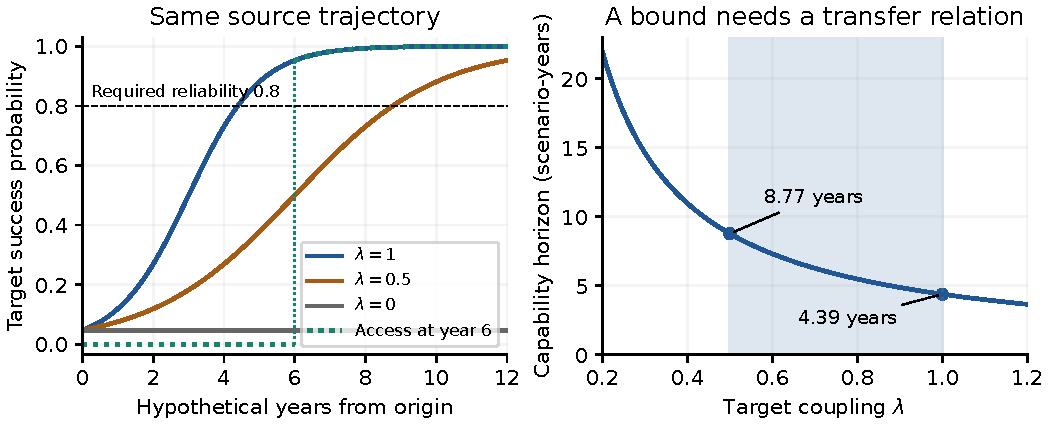
\includegraphics[width=\linewidth]{figures/capability_horizons.pdf}
\caption{Constructed capability horizons, not scientific forecasts. All four scenarios share the source path $x(t)-x_0=t$. Left: target success under strong coupling ($\lambda=1$), weaker coupling ($.5$), no coupling ($0$), or strong coupling with required access unavailable until year 6. The access-gated scenario starts at zero; the other three start at $.0474$. Right: horizon sensitivity to positive $\lambda$ at $q=.8$, $v=1$ and $\eta_0=-3$. The shaded range corresponds to the stipulated bound $\lambda\in[.5,1]$, not a statistical confidence interval. A calendar interpretation requires evidence for these parameters and the growth path.}
\label{fig:horizons}
\end{figure}

\paragraph{Capability and completion reversal.}
For independent serial attempts of duration $d$ and success probability $p>0$ launched at $s$, the number of attempts to first success is geometric, with mean $1/p$. Expected completion is therefore $s+d/p$. In the main assay example, launching A and B at their respective availability dates gives means $\tau_A+4/.8\approx9.39$ and $\tau_B+.25/.8\approx9.09$ scenario-years. Subtracting the two means shows that B finishes earlier on average exactly when $d_A-d_B>q(\tau_B-\tau_A)$, because both deployed versions have fixed success $q$. This compares two separate deployment choices. Adding B as an optional procedure does not force an optimal policy to abandon A; the policy can retain whichever choice is preferable. The validation durations and response curves are stipulated, not measured biomedical forecasts.

\section{Campaign reliability and the cost of evidence}
\label{sec:yield}
The following analyses connect target success probabilities to a concrete adoption decision. They show how a target-response probability enters experimental resource requirements and how uncertain that response may remain. Their stipulated parameters cannot be substituted for the source--target coefficients in the main horizon example.

\subsection{When is more reasoning worth its cost?}
Consider a deliberately simplified candidate-selection procedure. Each attempt costs $c$ units to propose a candidate and $v$ units to test it. Both are hypothetical monetary costs, not time; shared setup costs are set to zero. Let $p(c)$ be the probability that a proposed candidate meets the declared binding and cell-assay criteria after validation. The notation allows reasoning expenditure to affect yield but does not assume that it improves it. Hold the target and testing protocol fixed, and assume independent candidate outcomes with this same probability, where $0<p(c)<1$.

To find at least one validated hit with probability at least $\rho$, where $0<\rho<1$, reserve enough budget for $n$ attempts. Failure on all attempts has probability $(1-p(c))^n$. Thus the smallest attempt cap and its budget are
\begin{equation}
 n_\rho(c)=\left\lceil\frac{\log(1-\rho)}{\log(1-p(c))}\right\rceil,
 \qquad B_\rho(c)=n_\rho(c)(c+v).
 \label{eq:yieldbudget}
\end{equation}
This standard repeated-trial calculation gives the reserved budget for this procedure; stopping after a hit can spend less. It does not estimate elapsed time or optimize over other methods.

\begin{table}[htbp]
\caption{Hypothetical choices for reaching at least 90\% probability of one validated hit. Assay cost $v=9$ in every row; outcomes are independent with constant yield. Shared activity, batch effects or adaptive selection can violate this model. Costs share arbitrary monetary units; setup is excluded here. Yields are stipulated, not estimates from cited studies.}
\label{tab:yield}
\centering\small
\begin{tabular}{lrrrr}
\toprule
Procedure & Proposal cost $c$ & Hit probability $p$ & Attempts $n$ & Budget $B$\\
\midrule
Baseline & 1 & 0.10 & 22 & 220\\
Cheaper proposals & 0.1 & 0.10 & 22 & 200.2\\
Better selection & 2 & 0.20 & 11 & 121\\
Costlier, unchanged yield & 2 & 0.10 & 22 & 242\\
\bottomrule
\end{tabular}
\end{table}

Table~\ref{tab:yield} shows the decision. Tenfold cheaper proposals save 9\% of the campaign budget. Doubling proposal expenditure while doubling validated yield saves 45\%, because fewer assays are needed. Doubling expenditure without improving yield instead raises the budget by 10\%. Neither cheaper computation nor a higher source benchmark score determines which row applies. That requires evidence about $p(c)$ on the biomedical target.

\paragraph{The threshold that changes the decision.}
At a new per-attempt cost of 11, a strict saving over the baseline budget 220 permits at most 19 attempts. Reaching $\rho=.9$ therefore requires $p\ge1-.1^{1/19}\approx.1141$. The yield need not double: increasing it from .10 to at least .1141 suffices under this model. A pilot should resolve whether the new procedure clears that threshold, rather than merely whether its source score improves. Uncertainty matters: a point estimate above the threshold is not a reliability guarantee. Appendix~\ref{app:yield} propagates a yield interval into budget bounds.


Independence is not essential for a sufficient guarantee. If each candidate succeeds with conditional probability at least $p_{\min}$ after every reached failure history, the chain rule bounds $n$ consecutive failures by $(1-p_{\min})^n$. The same attempt cap is then sufficient, though not necessarily minimal. An average marginal yield is weaker: if all candidates share one binary outcome, repeated tests never raise success above $p$. An expert-filtered selector has a yield conditional on that whole selection procedure, not on raw proposals. Adaptive selection can also change yield after each observation. Neither selected-hit counts nor average marginal yield alone supply the history-conditional guarantee.

\subsection{A published case: what is measured, and what is missing?}
\begin{table}[htbp]
\caption{Connecting capability evidence to a scientific endpoint: a bounded audit of Co-Scientist Fig.~2a and initial AML Fig.~3a--c. Unknown entries identify measurements needed for the forecast, not evidence of zero benefit.}
\label{tab:transferrecord}
\centering\small
\begin{tabular}{P{.22\linewidth}P{.70\linewidth}}
\toprule
Field & Reported evidence and supported boundary\\
\midrule
Source measurement & Top-hypothesis Elo ratings rise across ten temporal buckets covering 203 research goals (Fig.~2a); ratings are relative comparisons, not assay probabilities.\\\addlinespace[3pt]
Biomedical target & Initial AML repurposing: cell-viability inhibition (Fig.~3a--c), distinct from the hypothetical binding-plus-cell-activity target in this appendix and from clinical benefit.\\\addlinespace[3pt]
Selection and people & Oncologists selected five drugs from thirty ranked candidates before testing; expert filtering is part of the procedure.\\\addlinespace[3pt]
Matched baseline & These results do not pair each reasoning budget with a matched laboratory arm and baseline procedure.\\\addlinespace[3pt]
Outcome denominator & Three of five selected drugs showed reported inhibition. This does not estimate unfiltered generator yield or how yield changes with reasoning budget.\\\addlinespace[3pt]
Costs and decision & Complete matched campaign costs and reuse savings are not identified by these results. Unknown benefit is not zero benefit.\\
\bottomrule
\end{tabular}
\end{table}
\label{sec:case}
Co-Scientist reports both computational scaling and laboratory outcomes \citep{gottweis2026coscientist}. Table~\ref{tab:transferrecord} records what connects its hypothesis-ranking result to its initial acute myeloid leukemia (AML) drug-repurposing experiment. The six fields distinguish the source measurement, target, adapter, baseline, outcomes and costs. They document the narrower workflow comparison; they are not a replacement for capability-to-target calibration.



The combined system-and-expert workflow produced active candidates. The authors distinguish this early validation from clinical efficacy. What remains unmeasured here is how changing the source capability changes yield and cost under a fixed selection-and-testing protocol. The table states the scope of this audit.

\paragraph{Why the missing comparison matters.}
Even knowing a new procedure's yield need not settle adoption. Stipulate its yield is .20 and each attempt costs 11: its .9-reliability budget is 121. If baseline yield is .10 at cost 10, the baseline budget is 220 and adoption saves money. If baseline yield is .30 at the same cost, its budget is 70 and adoption costs more. Both worlds agree on the new procedure's results. An unmeasured baseline therefore leaves even the direction of savings unresolved. These are constructed worlds, not estimates for Co-Scientist.

The pilot below uses complete outcome denominators and explicit uncertainty under its stipulated observation model. A discovery-stage claim needs validation of its declared endpoint, not a clinical trial unless patient benefit is claimed.


\subsection{Propagating uncertainty into campaign reserves}
\label{app:yield}
\paragraph{How uncertainty changes the budget.}
For a fixed independent-attempt procedure, $B_\rho(p)$ decreases as $p$ increases. Thus a valid interval $0<p_L\le p\le p_U<1$ implies
\begin{equation}
 (c+v)\left\lceil\frac{\log(1-\rho)}{\log(1-p_U)}\right\rceil
 \le B_\rho(p)\le
 (c+v)\left\lceil\frac{\log(1-\rho)}{\log(1-p_L)}\right\rceil.
 \label{eq:yieldinterval}
\end{equation}
For measured $p$, use a lower confidence bound appropriate to the prespecified sampling and selection procedure. On the event that it covers the true fixed $p$, substituting that bound provides the stated conditional campaign guarantee. Confidence coverage and campaign reliability are separate probabilities and should be reported separately; a .9 reliability target is not automatically a .9 unconditional guarantee after estimation. A zero lower bound gives no finite cap through this argument. An ordinary binomial interval for a marginal yield cannot establish the uniform history-conditional bound needed by an adaptive policy. If both procedures' yields or costs are uncertain, propagate both; robust savings require the new upper budget bound below the baseline lower bound.

\subsection{Exact decision analysis for a fixed pilot}
\label{sec:pilot_analysis}
\label{app:pilot}
This analysis asks how much evidence the proposed comparison can require, within the same hypothetical campaign model. It does not estimate biological yields or validate the reporting framework against real teams. The analysis contract was saved before outcomes: two frozen procedures, baseline and candidate per-attempt costs 10 and 11, campaign reliability $\rho=.9$, pilot sizes $N\in\{25,50,100,250,500,1000\}$ per arm, baseline yield $.10$, and candidate yields $.08,.10,.12,.20,.30$. The range includes worse, unchanged, near-threshold and substantially improved procedures; all results are retained.

\paragraph{Pilot and future campaign are different stages.}
A pilot always completes its prespecified $N$ independent attempts in each arm; it does not stop at the first hit or choose its size from interim results. Each arm has a fixed unknown yield $p_j$ and known cost $a_j$, with $j=0$ for baseline and $j=1$ for candidate. For this calculation the arms are independent too. All selected attempts enter the denominator; validity and failure rules, target, candidate-selection procedure and assay are fixed in advance. The subsequent campaign seeks at least one hit and reserves $B_j(p)=a_j\lceil\log(1-\rho)/\log(1-p)\rceil$, with $B_j(0)=\infty$ and $B_j(1)=a_j$. Setup costs are zero here. Shared batches, adaptive candidate selection, changing yield or uncertain costs need another observation/cost model.

\paragraph{A conservative decision rule from standard intervals.}
Let $X_j\sim\mathrm{Binomial}(N,p_j)$. Give each arm an equal-tailed Clopper--Pearson interval $[L_j,U_j]$ with coverage at least $1-\alpha/2$, where $\alpha=.05$ \citep{clopper1934}. For count $0<x<N$, the endpoints are beta quantiles
\[
 L(x)=F^{-1}_{\mathrm{Beta}(x,N-x+1)}(\alpha/4),\qquad
 U(x)=F^{-1}_{\mathrm{Beta}(x+1,N-x)}(1-\alpha/4).
\]
Use $L(0)=0$, $U(N)=1$, and the same quantile formulas for the other endpoint at these extremes. With probability at least $1-\alpha$, both true yields are covered: apply the union bound to the two noncoverage events. Monotonicity then gives $B_j(U_j)\le B_j(p_j)\le B_j(L_j)$ simultaneously. Report
\[
 \begin{array}{ll}
 \text{adopt:} & B_1(L_1)<B_0(U_0),\\
 \text{non-saving:} & B_1(U_1)\ge B_0(L_0),\\
 \text{unresolved:} & \text{otherwise}.
 \end{array}
\]
On the joint coverage event either resolved conclusion is correct. Thus the unconditional probability of a wrong resolved conclusion is at most $\alpha$ for every pair of fixed yields under this model. This is not a 95\% probability of correctness conditional on selecting a conclusion, nor the future campaign's 90\% reliability. The guarantee is inherited confidence-interval reasoning, not a novel statistical method. The rule can be conservative; no optimality or comparison against all decision rules is claimed.

\paragraph{Exact enumeration and comparator.}
For each prespecified parameter setting, sum the decision indicator over all $(N+1)^2$ possible count pairs weighted by their independent binomial probabilities. The implementation evaluates equivalent binomial tails, with direct double-sum cross-checks at $N=25$. There are no random seeds, Monte Carlo error bars or fitted parameters. The point-estimate comparator adopts when $B_1(X_1/N)<B_0(X_0/N)$ and otherwise keeps the baseline. It uses identical observations and cost accounting, but has no stated error guarantee and never defers. Report adoption, non-saving, unresolved and wrong-decision probabilities, rather than comparing a selective rule only on its accepted cases. A separate numerical check over $N\in\{25,100,500\}$, $p_0\in\{.05,.10,.20\}$ and 41 equally spaced $p_1\in[.02,.40]$ verifies the error inequality at 369 settings; the analytical coverage argument, not that finite grid, establishes the guarantee.

\paragraph{Sensitivity to reliability and sampling error.}
\label{app:threshold_sensitivity}
Reliability $\rho$ is the desired chance of a future campaign hit; $\alpha$ bounds a wrong resolved decision over repeated pilots under the sampling model. They answer different questions. A retrospective exact sensitivity crosses $\rho\in\{.8,.9,.95\}$, $\alpha\in\{.01,.05,.10\}$ and candidate yields $p_1\in\{.10,.12,.20,.30\}$, with baseline yield $.10$, $N=100$ per arm and costs 10/11 fixed: 36 settings. All count pairs are weighted by independent binomial probabilities. At $\rho=.9$ and $p_1=.20$, adoption is .646\%, 4.572\% and 10.902\% as $\alpha$ increases; for unchanged yield, false adoption is .0005\%, .0182\% and .0714\%. At $\alpha=.05$ and doubled yield, adoption is 5.099\%, 4.572\% and 5.003\% across the three $\rho$ values. Integer campaign caps make these differences nonmonotone. Low power persists in this grid, but the grid neither justifies a user's threshold nor compares all decision rules. Thresholds should reflect the consequences of error and deferral; prespecification alone supplies no such justification. The standard-library implementation in \texttt{scripts/analyze\_pilot\_threshold\_sensitivity.py} inverts binomial tails, checks coverage and reproduces the original four overlapping settings to absolute error below $10^{-10}$. All 36 outcomes are retained; this is hypothetical analysis, not empirical confirmation.

\paragraph{Evaluation costs and boundaries.}
Pilot expenditure is $N(10+11)=21N$, charged separately from the future campaign. For the stipulated $.10\to.20$ improvement, future budgets fall from 220 to 121. If the entire pilot is charged as an additional expense and its own hits receive no credit, offsetting that expense in reserved-budget savings requires $\lceil21N/99\rceil$ otherwise identical future campaigns. This assumes the saving is known and realized in subsequent budget allocations; it is not an expected cash-payback calculation. Campaigns may stop early, so actual expenditure differs from the reserve. This is an accounting illustration, not an estimate of experimental prices or net scientific value. Pilot hits may themselves be valuable; deployment frequencies and task changes also matter. The comparison shows why an uncertainty-aware evaluation can be sound yet uneconomic for a one-off decision. Biological dependence or distribution change can invalidate the calculation; no amount of computation validates its premises.

\texttt{scripts/analyze\_decision\_pilot.py} saves every setting, checks interval endpoints against SciPy's exact binomial interval API, verifies campaign caps directly from success probabilities, and generates Figure~\ref{fig:pilot}. The complete build reruns these checks. This numerical analysis supports the implications of the stipulated model; a prospective matched study is still needed before claiming practical advantage in biomedical research.


\begin{table}[htbp]
\centering\small
\caption{All 30 prespecified hypothetical pilot settings. Baseline yield is $.10$ and its true .9-reliability campaign budget is 220; $B_1$ is the candidate's true budget. Costs are arbitrary monetary units. Adoption probabilities refer to repeated pilots under the stipulated yields. The interval rule may defer; the point-estimate rule does not. At $p_1\le.10$, adoption is erroneous. Percentages are rounded to three decimals; displayed zeros can be small positive probabilities. Pilot expenditure is separate from campaign reserves.}
\label{tab:pilotfull}
\begin{tabular}{rrrrrrr}
\toprule
$N$ & $p_1$ & $B_1$ & Interval adopt (\%) & Unresolved (\%) & Point adopt (\%) & Pilot cost\\
\midrule
25 & 0.08 & 308 & 0.000 & 99.994 & 30.720 & 525\\
25 & 0.10 & 242 & 0.001 & 99.996 & 40.456 & 525\\
25 & 0.12 & 209 & 0.003 & 99.995 & 49.851 & 525\\
25 & 0.20 & 121 & 0.157 & 99.843 & 78.978 & 525\\
25 & 0.30 & 77 & 2.412 & 97.588 & 95.106 & 525\\
\midrule
50 & 0.08 & 308 & 0.001 & 99.934 & 29.846 & 1050\\
50 & 0.10 & 242 & 0.006 & 99.969 & 43.245 & 1050\\
50 & 0.12 & 209 & 0.023 & 99.967 & 56.165 & 1050\\
50 & 0.20 & 121 & 0.911 & 99.089 & 89.335 & 1050\\
50 & 0.30 & 77 & 12.630 & 87.370 & 99.094 & 1050\\
\midrule
100 & 0.08 & 308 & 0.003 & 99.630 & 25.069 & 2100\\
100 & 0.10 & 242 & 0.018 & 99.900 & 41.877 & 2100\\
100 & 0.12 & 209 & 0.088 & 99.895 & 58.853 & 2100\\
100 & 0.20 & 121 & 4.572 & 95.428 & 95.801 & 2100\\
100 & 0.30 & 77 & 46.899 & 53.101 & 99.952 & 2100\\
\midrule
250 & 0.08 & 308 & 0.001 & 98.704 & 13.432 & 5250\\
250 & 0.10 & 242 & 0.013 & 99.836 & 36.103 & 5250\\
250 & 0.12 & 209 & 0.170 & 99.817 & 63.892 & 5250\\
250 & 0.20 & 121 & 28.697 & 71.303 & 99.687 & 5250\\
250 & 0.30 & 77 & 96.783 & 3.217 & 100.000 & 5250\\
\midrule
500 & 0.08 & 308 & 0.000 & 95.678 & 5.694 & 10500\\
500 & 0.10 & 242 & 0.008 & 99.694 & 29.528 & 10500\\
500 & 0.12 & 209 & 0.299 & 99.692 & 68.445 & 10500\\
500 & 0.20 & 121 & 71.254 & 28.746 & 99.994 & 10500\\
500 & 0.30 & 77 & 99.996 & 0.004 & 100.000 & 10500\\
\midrule
1000 & 0.08 & 308 & 0.000 & 83.945 & 1.242 & 21000\\
1000 & 0.10 & 242 & 0.004 & 99.281 & 22.175 & 21000\\
1000 & 0.12 & 209 & 0.630 & 99.365 & 75.618 & 21000\\
1000 & 0.20 & 121 & 98.503 & 1.497 & 100.000 & 21000\\
1000 & 0.30 & 77 & 100.000 & 0.000 & 100.000 & 21000\\
\bottomrule
\end{tabular}

\end{table}
\FloatBarrier
\begin{figure}[htbp]
\centering
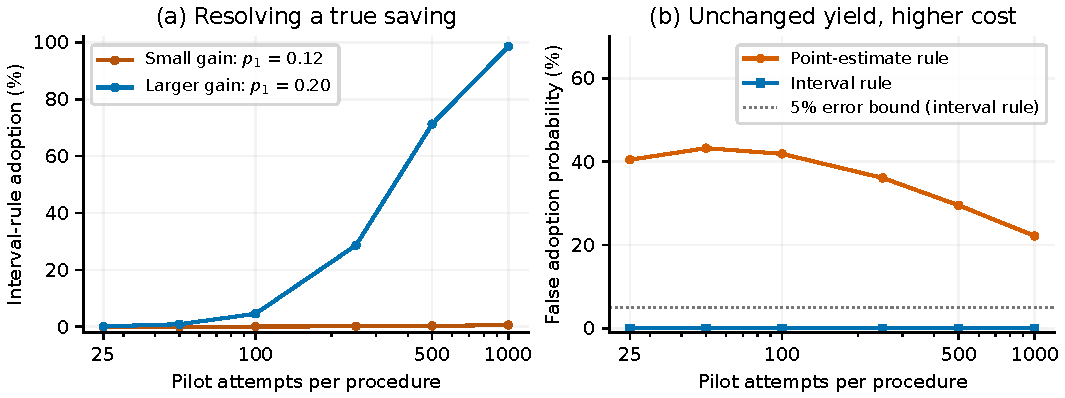
\includegraphics[width=\linewidth]{figures/decision_pilot.pdf}
\caption{Exact hypothetical pilot analysis. Baseline yield is $.10$, per-attempt costs are 10 and 11, and future campaign reliability is $.9$. Left: probability of recommending adoption when a true saving exists. The interval rule requires the candidate upper budget bound below the baseline lower bound. Right: probability of false adoption when yield is unchanged and costs rise; the two panels answer different questions. Lines join evaluated sizes, not a fitted scaling law. Neither rule is claimed optimal.}
\label{fig:pilot}
\end{figure}
\section{Foundations and further research directions}
\label{sec:related}
Computational discovery builds on models of law and concept discovery \citep{langley1987}, reliable inquiry \citep{kelly1996}, and transformative discoveries in knowledge networks \citep{chen2009discovery}. Information-based complexity combines costly observations with computation \citep{traub1988,werschulz2002}. We build on these foundations to study the evolving reach of AI research procedures.

\begin{table}[htbp]
\centering\small
\caption{Closest predictive foundations and the remaining scientific question. The right column states obligations for our programme, not established advantages.}
\label{tab:foundations}
\begin{tabular}{P{.26\linewidth}P{.31\linewidth}P{.34\linewidth}}
\toprule
Foundation & Established construction & Additional question here\\
\midrule
Observational scaling \citep{ruan2024} & Shared capability coordinates predict downstream performance. & Which target requirements improve prediction beyond these coordinates?\\\addlinespace[3pt]
Demand and response scales \citep{zhou2026scales,truong2026irsl} & Model ability and item demands jointly determine responses. & Which descriptors transport to unseen research targets?\\\addlinespace[3pt]
Task-duration horizons \citep{kwa2025}; compute scenarios \citep{whitfill2025} & Estimate reliable task duration and condition its growth on resources. & What extra relation connects that ability to a specified scientific endpoint?\\\addlinespace[3pt]
Information complexity and workflow analysis \citep{werschulz2002,meyerson2025} & Account for observation access, computation and dependencies. & How do changed procedures alter capability and completion times separately?\\
\bottomrule
\end{tabular}
\end{table}

Measurement validity is part of this question. \citet{wallach2025} distinguish conceptualization from operational measurement; \citet{zhuang2025} advocates psychometric evaluation, and \citet{chollet2019} emphasizes priors and generalization difficulty. A descriptor needs a defensible meaning as well as predictive accuracy. Cost-controlled agents and reproducible research environments supply relevant evaluation practice \citep{kapoor2024,bragg2026astabench}.

Scientific scaling is already an agenda \citep{zhang2025discovery,ye2026v2}, alongside resource-constrained automation and scientific-pathway forecasting \citep{luo2026,chamoun2026}. Data-stock forecasts illustrate uncertainty under resource scenarios \citep{villalobos2024}; scientific event forecasting differs empirically from scientific reasoning \citep{wu2026forecasting}. Our question is which measurements justify moving from capability to target performance, then to a date. Neither logistic fitting nor computational discovery is new.


Learned representations can change experimental search \citep{rankovic2026}, and discovery loops can use evaluated histories \citep{ye2026v2}. Recursive self-improvement may alter capability growth or procedure-development costs \citep{zhang2026dgm,zhang2026hyperagents}. A successful cycle supports that cycle; sustained acceleration requires measurements across successive improvements and their full costs.


\section{An exploratory finite experimental-table forecast screen}
\label{app:finite_table}
We test the proposed next step on public tables distributed with GOLLuM \citep{rankovic2026}: four additive-screening plates, five Buchwald--Hartwig reaction tables, one Suzuki--Miyaura table and one C2-yield table. These are eleven tables from four source families, not eleven independent scientific domains. The repository snapshot is pinned in the artifact. Its Apache license is retained; underlying experimental provenance remains attributed to the source study. We do not rerun the laboratory experiments or reproduce GOLLuM's language-model optimizer.

The original replay target was an observed objective at or above the admitted table's 90th percentile. All predictors received that threshold. After dropping incomplete and duplicate input rows, we uniformly subsampled at most 512 candidates without consulting outcomes. All eleven admitted sets contain 512 candidates. Numeric inputs are scaled by catalogue ranges and strings treated as categorical identities; outcome, procedure text and derived-output columns are excluded. The percentile uses the admitted archive to define a benchmark target, not information proved available to a historical forecaster. Ties and source dependence are reported in the retained metadata.

We ran 50 seeded campaigns per table. Five initially uniform observations were followed by a fixed Gaussian-process upper-confidence policy, with acquisition mean plus one posterior standard deviation, noise .01 and kernel $\exp(-2d)$, where $d$ averages squared normalized numeric differences and categorical mismatches. Standardization of outcomes uses only observations already revealed. Every measured candidate costs one unit; observations within the pilot count against the total budget. No language-model training or paid inference is performed.

At 5 and 10 observations, we predicted at least one hit by budget 20 (primary) or 40 (sensitivity). We compared ridge-logistic forecasts using budget alone, adding catalogue size, adding the best observed gap to threshold, and adding pilot mean, dispersion and pairwise kernel similarity. Catalogue size cannot differentiate these equally sized sets.

For pilot outcomes $y_i$ and supplied threshold $u$, let $s=\max\{|u|,\operatorname{sd}(y_i),10^{-8}\}$, using population standard deviation. Best gap, mean gap and dispersion are $(\max_i y_i-u)/s$, $(\bar y-u)/s$ and $\operatorname{sd}(y_i)/s$. Similarity averages the off-diagonal kernel entries among pilot candidates. These calculations use revealed outcomes and the known catalogue.

All predictors assign probability one after an observed pilot hit; logistic fits use only training campaigns without such a hit. The 550 campaigns yield 2,200 prefix--budget records (two prefixes and two budgets), evaluated by four predictors; these are repeated views of the same campaigns, not 8,800 independent trials. At pilot five, 221 campaigns have already hit and 329 remain. All other features use only the pilot and declared threshold; held-out future outcomes are evaluation labels. Each evaluation withheld an entire source family, keeping all five Buchwald--Hartwig tables or all four additive plates together. Forecast features were standardized on training families only. Losses were averaged equally within tables and then across source families, with the not-yet-hit stratum retained separately.

\begin{table}[htbp]\centering\small
\caption{Held-out-family Brier scores after five pilot observations, predicting success by budget 20. Lower is better. All forecasts use the same 550 campaign traces; pilot discoveries count as successes.}
\label{tab:finite_table}
\begin{tabular}{lrrr}
\toprule
Source family & Budget-only & + best gap & + pilot summaries\\
\midrule
additives & 0.00107 & 0.00175 & 0.00307\\
buchwald--hartwig & 0.01186 & 0.01213 & 0.01208\\
c2--yield & 0.01931 & 0.01971 & 0.01980\\
suzuki--miyaura & 0.03868 & 0.03946 & 0.03950\\
\bottomrule
\end{tabular}

\end{table}

Across families, budget-only Brier score is .01773, adding the best gap gives .01826, and pilot summaries give .01862. Thus the additional pilot descriptors do not improve the primary score. On campaigns without an initial hit, scores are .03106, .03197 and .03253. By budget 20 the family-averaged hit rate is 98.2\%; all retained campaigns have a hit by budget 40. This ceiling leaves little uncertainty for a discoverability forecast to resolve. The result neither validates the proposed descriptor nor establishes equivalence or impossibility; it identifies an uninformative easy-target regime for this screen. The stricter-endpoint analysis below is exploratory: its endpoints were chosen after this primary result was known.

For reference, uniform sampling without replacement from a table with $N$ candidates and $H$ archive hits has hit probability $1-\binom{N-H}{b}/\binom{N}{b}$ by budget $b$. The artifact retains this oracle-informed reference using full-table hit counts; it is not a forecast of the adaptive policy.

The artifact includes all candidate IDs, observed paths, source hashes, forecast features, fold predictions, per-table losses and calibration bins. Unique-query and future-outcome permutation checks protect the observed-prefix protocol. Four heterogeneous source families do not justify a calibrated target-population interval. This retrospective table replay supplies neither an intervention test of AI capability nor an information-available-at-the-time discovery forecast. A subsequent study would need a new independently fixed endpoint with substantial unresolved outcomes and held-out target families, not a redefinition selected to improve these scores.

\subsection{Exploratory comparisons with simple forecasts}
\label{app:replay_baselines}
Near-universal success can make a low Brier score easy to obtain. We therefore added three reference forecasts after seeing the original replay: always predict success; predict success only if the pilot already found a hit; and use success prevalence from training families. These reuse every campaign and the original endpoint. They are a retrospective challenge, not independent confirmation.

For the prevalence forecast, withhold the whole test source family. At each pilot/budget setting, use only other families' campaigns without a pilot hit; average their binary outcomes within tables, then tables within families and families equally. Assign this rate to unresolved test campaigns and probability one to those already known to have hit. Every fit retains three training families; no empty training stratum occurs. The always-success forecast uses no fitted parameters. The observed-hit-only forecast represents no further progress after the pilot, not a proposed competitive method.

Table~\ref{tab:replay_baselines} compares Brier score with log-loss, which penalizes confident errors more heavily. Both use the original scoring convention: clip probabilities to $[10^{-6},1-10^{-6}]$, average campaigns within tables, then tables within families, then families equally. The all-campaign column includes 550 campaigns; the no-pilot-hit column includes 329. Training prevalence nearly matches the budget-only logistic forecast. Always-success also nearly matches its Brier score but has substantially worse log-loss: rare failures contradict its near-certainty. The two metrics therefore expose different weaknesses. Neither result validates a prospective discovery forecast.

\begin{table}[htbp]\centering\small
\caption{Post-result baseline challenge at pilot five and budget 20. Lower is better for both losses. All rows use identical campaign outcomes and family/table weighting; the three added references are marked *. The two strata overlap and are not replications.}
\label{tab:replay_baselines}
\begin{tabular}{lrrrr}
\toprule
& \multicolumn{2}{c}{All campaigns} & \multicolumn{2}{c}{No pilot hit}\\
Forecast & Brier & Log-loss & Brier & Log-loss\\
\midrule
Budget-only logistic & 0.01773 & 0.08549 & 0.03106 & 0.14865\\
+ pilot summaries & 0.01862 & 0.10181 & 0.03253 & 0.17661\\
Training prevalence* & 0.01774 & 0.08571 & 0.03109 & 0.14900\\
Always success* & 0.01800 & 0.24868 & 0.03160 & 0.43654\\
Observed hit only* & 0.57025 & 7.87830 & 0.96840 & 13.37897\\
\bottomrule
\end{tabular}

\end{table}

The comparison covers all four pilot/budget settings, both strata and each source family. Numerical checks reproduced the original scores; perturbing held-out outcomes left fitted predictions unchanged, confirming their exclusion from fitting. These checks use the same 550 campaigns and provide no additional evidence of generalization to new sources.

\subsection{Endpoint sensitivity and source-level contrasts}
\label{app:endpoint_sensitivity}
Following the 98.2\% hit rate at the 90th-percentile endpoint, we chose stricter 95th- and 99th-percentile thresholds for an exploratory analysis. Their forecast scores were computed afterward. All 550 saved forty-step paths are reused without rerunning or changing the selection policy. Each endpoint redefines pilot-hit status, future-hit labels and the threshold-relative features. We refitted the same ridge-logistic budget and summary predictors with training-only standardization and leave-one-source-group exclusion. The existing best-gap predictor was then added as a simpler challenge to the 99th-percentile gain. All thresholds remain full-table hindsight information. This ordering makes the follow-up exploratory; it is not a new confirmation set.

Tables~\ref{tab:endpoint_full} and~\ref{tab:endpoint_family} retain all endpoint/pilot/budget comparisons and the primary source differences. Within each fold, the training-only prevalence reference balances tables and source groups among no-hit pilots and assigns one to already-hit pilots. Scores average campaigns within tables, tables within source groups, and the four groups equally, as in the original experiment. The same campaign appears in several rows; rows are not independent experiments.

\begin{table}[htbp]\centering\small
\caption{Endpoint sensitivity: family-balanced Brier scores. All three targets, two pilots, two budgets, four predictors and both strata are retained. The two strata overlap. Lower is better.}
\label{tab:endpoint_full}
\begin{tabular}{llrrrr}
\toprule
Percentile & Pilot/budget & Budget & Best gap & Summaries & Prevalence\\
\midrule
\multicolumn{6}{l}{All campaigns}\\
90 & 5/20 & 0.01773 & 0.01826 & 0.01862 & 0.01774\\
90 & 5/40 & 0.00000 & 0.00000 & 0.00000 & 0.00000\\
90 & 10/20 & 0.01730 & 0.01768 & 0.01786 & 0.01734\\
90 & 10/40 & 0.00000 & 0.00000 & 0.00000 & 0.00000\\
95 & 5/20 & 0.09346 & 0.10043 & 0.10460 & 0.09418\\
95 & 5/40 & 0.00503 & 0.00514 & 0.00515 & 0.00504\\
95 & 10/20 & 0.08097 & 0.08762 & 0.09705 & 0.08119\\
95 & 10/40 & 0.00509 & 0.00508 & 0.00519 & 0.00507\\
99 & 5/20 & 0.28716 & 0.34035 & 0.16489 & 0.28510\\
99 & 5/40 & 0.22316 & 0.22688 & 0.29591 & 0.22966\\
99 & 10/20 & 0.21259 & 0.24759 & 0.14558 & 0.21475\\
99 & 10/40 & 0.23235 & 0.23634 & 0.27048 & 0.22517\\
\multicolumn{6}{l}{No pilot hit}\\
90 & 5/20 & 0.03106 & 0.03197 & 0.03253 & 0.03109\\
90 & 5/40 & 0.00000 & 0.00000 & 0.00001 & 0.00000\\
90 & 10/20 & 0.09101 & 0.09376 & 0.09401 & 0.09089\\
90 & 10/40 & 0.00002 & 0.00001 & 0.00002 & 0.00000\\
95 & 5/20 & 0.11963 & 0.12798 & 0.13341 & 0.12071\\
95 & 5/40 & 0.00599 & 0.00613 & 0.00614 & 0.00600\\
95 & 10/20 & 0.21364 & 0.23029 & 0.25620 & 0.21459\\
95 & 10/40 & 0.01277 & 0.01274 & 0.01303 & 0.01271\\
99 & 5/20 & 0.30416 & 0.36056 & 0.17473 & 0.30196\\
99 & 5/40 & 0.23720 & 0.24108 & 0.31476 & 0.24408\\
99 & 10/20 & 0.26740 & 0.30743 & 0.18903 & 0.26974\\
99 & 10/40 & 0.26631 & 0.27181 & 0.29886 & 0.25758\\
\bottomrule
\end{tabular}

\end{table}

\begin{table}[htbp]\centering\small
\caption{Paired Brier difference, summaries minus budget-only, at pilot five/budget 20. Negative favors summaries. These are four descriptive source contrasts, not independent draws from a specified scientific population.}
\label{tab:endpoint_family}
\begin{tabular}{lrrr}
\toprule
Source & 90th & 95th & 99th\\
\midrule
Additive screens & +0.00201 & +0.02455 & -0.17351\\
Buchwald--Hartwig & +0.00022 & +0.00714 & -0.06007\\
C2-yield & +0.00050 & +0.00172 & -0.11672\\
Suzuki--Miyaura & +0.00083 & +0.01113 & -0.13881\\
\bottomrule
\end{tabular}

\end{table}

At the 99th percentile, pooled log-loss falls from .76525 to .49995; the best-gap and prevalence references score .88142 and .76174. At the 95th percentile it worsens from .31881 to .38814. Omitting any one source from the average of the existing held-out losses gives 99th-percentile Brier differences from $-.14301$ to $-.10520$. This is reweighting of fixed fold results, not refitting with only two training sources. No target-population confidence interval is claimed. The no-pilot-hit 99th-percentile score also improves, from .30416 to .17473. Gains cannot be attributed solely to the deterministic already-hit gate. They do not persist at the forty-observation budget: at pilot five, summaries score .29591 versus .22316 for budget-only; at pilot ten, .27048 versus .23235. Thus the follow-up identifies an endpoint-and-budget-specific contrast, not uniform summary superiority.

An independent solver reproduced the original predictions, and held-out-label perturbations left fitted predictions unchanged; source-file identities and thresholds were also checked. The saved 26,400 forecast records reuse the same 550 campaign histories and include every table/group loss and log-loss summary. The endpoint-dependent reversal warrants prospective testing of what early observations predict; it does not establish an AI-capability effect, clinical utility or a fitted discovery date.


\subsection{Budget-specific forecasts and opposing source errors}
\label{app:horizon_diagnostic}
The longer-budget reversal admits a simple rival explanation: perhaps one set of summary coefficients cannot describe both budgets. We tested this after the endpoint analysis, retaining all three endpoints, both pilots, both budgets and the same four source exclusions. No trajectories or outcomes were added. The shared model is the original logistic regression. Separate models fit each budget independently, using both pilot lengths. For each held-out source, feature centering and scaling are still computed on the complete outer training set, so changing budgets does not also change feature units. Budget is constant within a separate fit; its penalized coefficient is zero. The best-gap predictor receives the same comparison.

The primary separate fits retain penalty 1. Each budget has half as many training rows, so a second control uses penalty $n_h/n_{\rm pool}=1/2$: with weights summing to the training-row count, this preserves the penalty per weighted observation. Intercepts remain unpenalized. This changes coefficient sharing and parameter count; it is neither a new forecasting algorithm nor an isolated causal intervention on information. The same deterministic probability-one rule applies after a pilot hit. Predicted probabilities are clipped to $[10^{-6},1-10^{-6}]$ for both losses, as in the original analysis.

\begin{table}[htbp]\centering\small
\caption{Exploratory forecast-specification check. Brier scores use all campaigns and equal source/table weighting. Shared: original coefficients across budgets. Separate: independent budget fits, penalty 1. Matched: separate fits with penalty $1/2$. All endpoints, pilots and budgets are shown; these are repeated forecasts of the same 550 histories.}
\label{tab:horizon_specification}
\begin{tabular}{lrrrrrrrr}
\toprule
Endpoint & Pilot & Budget & \multicolumn{3}{c}{Budget-only} & \multicolumn{3}{c}{Summaries}\\
 & & & Shared & Separate & Matched & Shared & Separate & Matched\\
\midrule
90 & 5 & 20 & 0.01773 & 0.01774 & 0.01774 & 0.01862 & 0.01872 & 0.01874\\
90 & 5 & 40 & 0.00000 & 0.00000 & 0.00000 & 0.00000 & 0.00000 & 0.00000\\
90 & 10 & 20 & 0.01730 & 0.01735 & 0.01737 & 0.01786 & 0.01791 & 0.01784\\
90 & 10 & 40 & 0.00000 & 0.00000 & 0.00000 & 0.00000 & 0.00000 & 0.00000\\
95 & 5 & 20 & 0.09346 & 0.09340 & 0.09341 & 0.10460 & 0.10526 & 0.10533\\
95 & 5 & 40 & 0.00503 & 0.00504 & 0.00504 & 0.00515 & 0.00607 & 0.00671\\
95 & 10 & 20 & 0.08097 & 0.08096 & 0.08095 & 0.09705 & 0.09944 & 0.09954\\
95 & 10 & 40 & 0.00509 & 0.00507 & 0.00508 & 0.00519 & 0.00513 & 0.00522\\
99 & 5 & 20 & 0.28716 & 0.28494 & 0.28495 & 0.16489 & 0.15424 & 0.15423\\
99 & 5 & 40 & 0.22316 & 0.22607 & 0.22606 & 0.29591 & 0.33922 & 0.34428\\
99 & 10 & 20 & 0.21259 & 0.21396 & 0.21395 & 0.14558 & 0.13438 & 0.13436\\
99 & 10 & 40 & 0.23235 & 0.22957 & 0.22958 & 0.27048 & 0.31398 & 0.32052\\
\bottomrule
\end{tabular}

\end{table}

At the 99th-percentile endpoint, pilot five and budget 20, separate summary fits improve Brier score from .16489 to .15424. At budget 40 they worsen it from .29591 to .33922; log-loss worsens from .99753 to 2.31803. The matched-penalty score is .34428 (log-loss 2.50883). The separate best-gap reference also worsens at budget 40 (.24185 versus the shared .22688). Separate fitting therefore does not remove the observed long-budget failure, but this check does not exclude other representations or calibration procedures.

True hits are nested: a history that hits by observation 20 also hits by 40. Across all three endpoints and both pilots, none of the three original predictors violates this ordering in its forecasts. Separate summary fits do so for 2/550 histories at the 95th percentile and 10/550 at the 99th, both at pilot five. Matching the penalty increases these counts to 5 and 16; the matched best-gap fit has one strict-endpoint violation. All other settings have zero. These alternative fits are diagnostic comparisons, not recommended coherent completion distributions.

The apparent agreement of the overall success-rate mean has a different limitation. For the original strict-endpoint summary forecast at pilot five/budget 40, the equally weighted source means are predictions .34964, .99113, .96927 and .96732, against observed rates 1, .976, .28 and .98 for additives, Buchwald--Hartwig, C2 and Suzuki--Miyaura. Underprediction and overprediction cancel: their averages are .81934 and .809. For each campaign, the residual is predicted hit probability minus its binary outcome. Within each table, mean squared residual equals squared mean residual plus residual variance. Averaging this identity by the scoring weights gives $.29591=.22732+.06860$; rounding accounts for the last digit. Thus 76.8\% of this descriptive error comes from within-table mean residuals. This is not a calibration guarantee or a population bias estimate; it diagnoses the existing predictions without fitting to held-out labels. Averaging sources before squaring would hide these opposing errors.

Checks reproduced all 19,800 original logistic predictions exactly and verified eleven source hashes, 180 held-out-label perturbations, nested outcomes and the error decomposition. Retained forecasts and losses cover both score strata and every source/table. The 59,400 records reuse 550 histories, not new experiments; independently chosen endpoints and sources remain necessary before generalizing.

\end{document}
